\chapter{基于数据分布感知激活值的子模型抽取联邦学习}
\label{sec:chapterfeddse}
\section{引言}

\subsection{神经元冲突现象}
在章节\ref{sec:sub-extract}详细介绍了联邦学习在资源受限情况
基于子模型抽取方向最新的研究,
都在解决资源受限的问题上提出了完整的解决方案。
这些解决方法的特点是基于提前预定好的抽取规则,
这些方案的一个严重的缺点是会造成\textbf{神经元冲突}。
图\ref{fig:3-1competion}作为例子具体介绍了冲突过程。
%ppppppppppppppppppppppppppppppppppppppp
\begin{figure}[thbp]
    \centering
    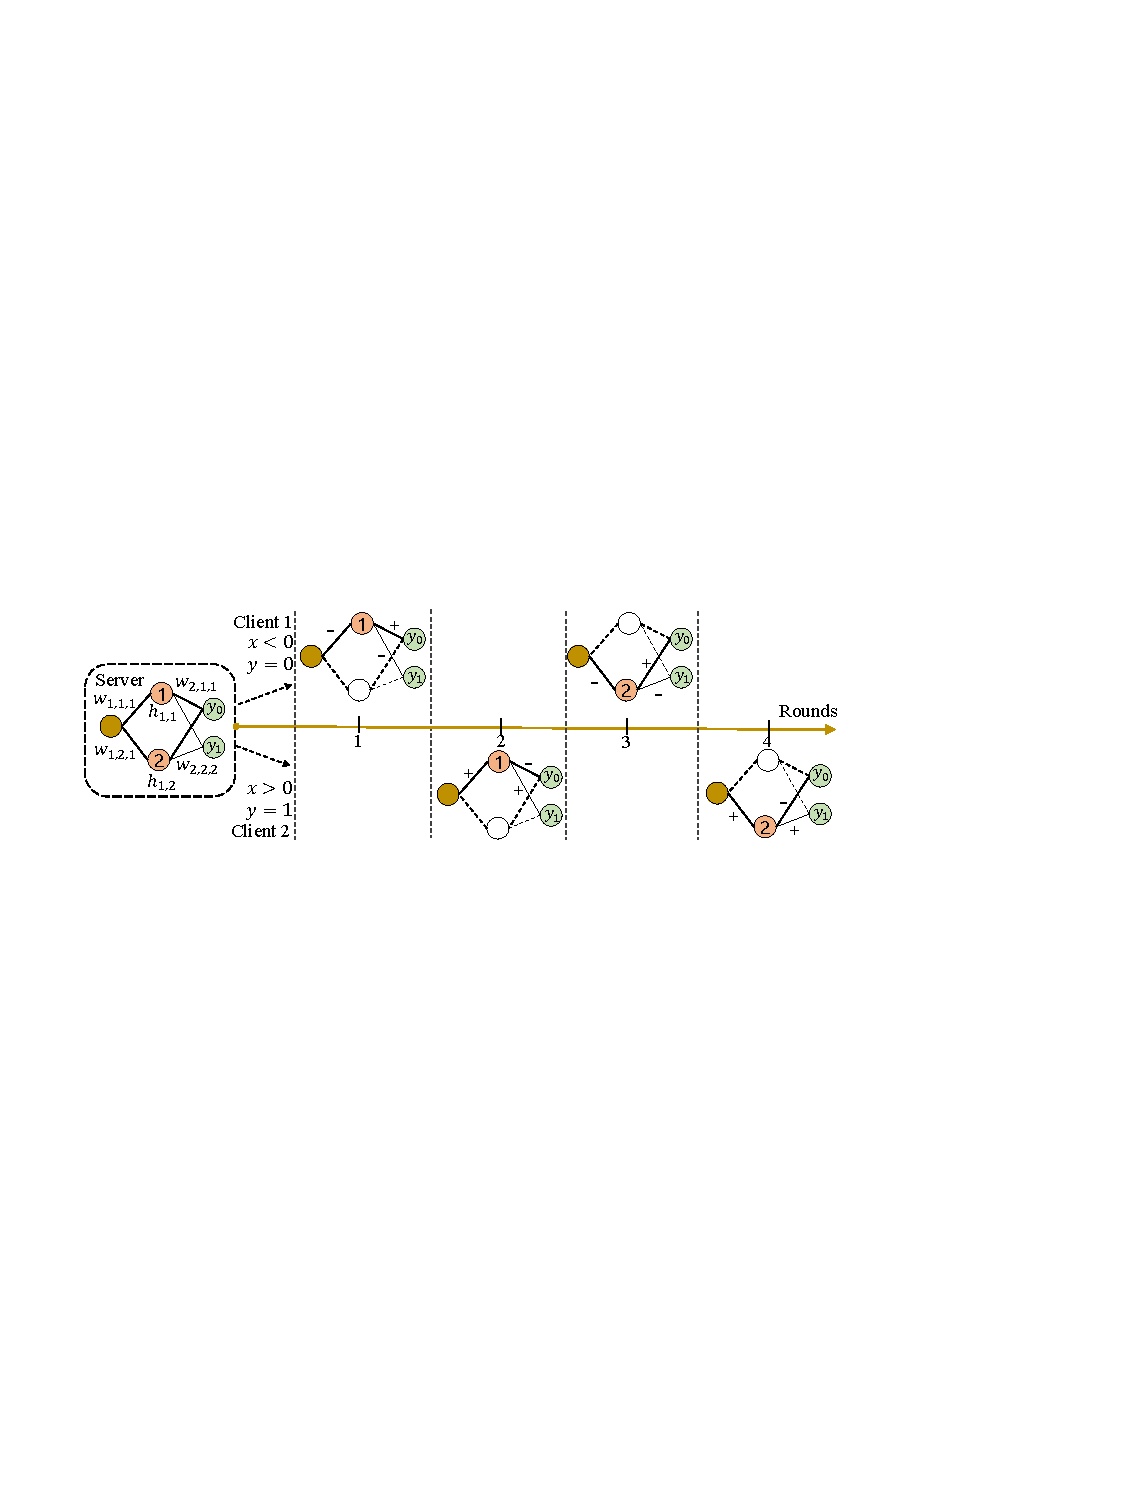
\includegraphics[width=0.9\linewidth]{chapter3/3-1-引言.pdf}
    \caption{\label{fig:3-1competion}当前方法引起神经元冲突}
\end{figure}
%ppppppppppppppppppppppppppppppppppppppp
图片中是一个拥有六个可训练参数的简单的深度学习神经网络,
图中参数分别为$W_{1, 1, 1}$、$W_{1, 2, 1}$、$W_{2, 1, 1}$、
$W_{2, 1, 2}$、$W_{2, 2, 1}$以及$W_{2, 2, 2}$六个参数,
这个神经元要训练一个网络根据$x$的不同$y$值输出$0$或者$1$。
我们假定存在两个客户Client 1和Client 2,
其中Client 1拥有的数据是$\{ x < 0 , y=0 \}$,
而Client 2中拥有的数据是$\{ x > 0 , y=1 \}$。
在第一轮中Client 1选择了编号为$1$的神经元训练,
因为$x<0$,要想使$y=0$也就是输出$y_{0}$的概率变大,
模型会朝着将$W_{1, 1, 1}<0, W_{2, 1, 1}>0$的方向上靠近,
这样保证$x$在分别与$W_{1, 1, 1}<0, W_{2, 1, 1}>0$相乘之后
输出的值是个很大的正数,
也就是选择神经元$y_0$也就是$y=0$的概率变大。
而在保证$W_{1, 1, 1}<0, W_{2, 1, 1}>0$的情况下,
保证$W_{2, 1, 2}<0$,
这样$x$在分别与$W_{1, 1, 1}<0, W_{2, 1, 2}<0$相乘之后
输出的值是个很小的数,
也就是选择神经元$y_1$也就是$y=1$的概率变小。
经过Client 1的训练之后,
可以得到$W_{1, 1, 1}<0, W_{2, 1, 1}>0, W_{2, 1, 2}<0$这样的结论,
如图\ref{fig:3-1competion}中的第一轮符号所示。
在第二轮的训练中,
Client 2抽取了与Client 1一样的子模型,
也就是选择了序号为$1$的神经元,
但是由于Client 2的数据是$\{ x > 0 , y=1 \}$,
正好与Clinet 1保持相反的数据分布,
要想使得在$x>0$的情况下,输出$y_1$也就是$y=1$的概率增大,
模型会朝着将$W_{1, 1, 1}>0, W_{2, 1, 1}<0$的方向上靠近,
这样保证$x$在分别与$W_{1, 1, 1}>0, W_{2, 1, 1}<0$相乘之后
输出的值是个很小的数,
也就是选择神经元$y_1$也就是$y=1$的概率变大。
同样的,
选择$W_{1, 1, 1}>0, W_{2, 1, 2}>0$
保证选择神经元$y_0$也就是$y=0$的概率变小。
这样在Client 2中得到了与Client 1相反的优化方向
$W_{1, 1, 1}>0, W_{2, 1, 1}<0, W_{2, 1, 2}>0$,
如图\ref{fig:3-1competion}中的第二轮符号所示。
按照联邦学习最后聚合的算法,
将Client 1与Client 2的参数进行聚合,
可以发现同一个神经元在两种不同的数据下出现了竞争的情况,
不同边缘设备数据将神经元按照不同甚至相反的方向优化,
这势必会造成训练效果的下降。

基于预先制定分配神经元方法所带来的神经元冲突问题,
可以观察在联邦学习中不同边缘设备带来不同的数据对全局模型
中激活神经元的分布情况,
来自适应的给不同的客户端分配子模型。

\subsection{分布现象观察}
为了观察不同数据在深度学习模型中激活神经元的分布,
设计了实验来观察不同激活值的现象。
我们设计了一个三层的多层感知机在数据集EMNIST上进行实验,
三层感知机神经元的数量分别是$50$、$24$以及$10$,
然后统计了在训练过程中每层神经元中的平均激活值。
这次联邦学习实验设定了五个客户端,
每个客户端分别包含两类别的数据。
具体的对比如图\ref{fig:compare-clients0}和图\ref{fig:compare-clients1}所示,
图中每行的layer1、layer2和layer3分别表示多层感知机的
第一层、第二层和第三层,
每个图标的横轴表示当前层的神经元的序号,
例如在layer1是$1-50$的序号,
纵坐标表示当前神经元在多个训练批次过程中的激活值的平均值,
每行图片比较了不同两个客户端之间的激活值之间分布的不同分布,
图\ref{fig:compare-clients0}和图\ref{fig:compare-clients1}
记录了所有两个客户端对比的数据。
通过观察不同层不同神经元激活值的分布可以观察看客户端之间存在的冲突。

观察图\ref{fig:compare-clients0}中的第一行的layer1图,
可以发现对于相同序列的神经元来说,
Client 0和Client 1激活程度十分不同,
两者几乎大部分神经元的激活值都是不同的,
体现在图中两条曲线基本不存在重合的地方,
例如编号$18$的神经元在Client 1中激活值的大小接近与$1$,
而在Client 0中激活值的大小却接近与$0$。
如果Client 0和Client 1同时优化layer1层的多层感知机,
势必在编号$18$的神经元出起冲突,
Client 0要求输出接近1,才能更好的预测,
而相反的是Client 1要求输出接近0才能更好的预测自己的数据,
这种情况在聚合的过程中必然对于Client 0和Client 1都是一种削弱的情况。

%ppppppppppppppppppppppppppppppppppppppp
\begin{figure}[thbp]
    \centering
    \begin{subfigure}[b]{\textwidth}
        \centering
        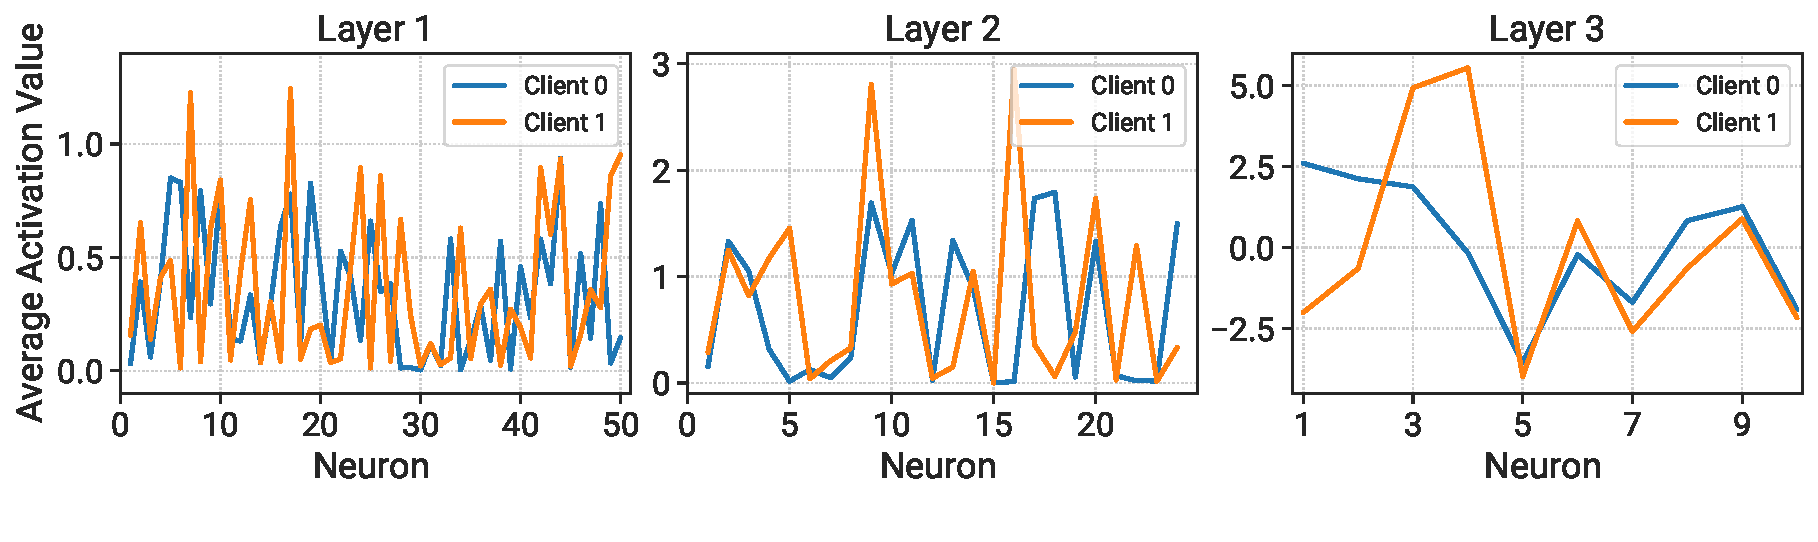
\includegraphics[width=0.95\linewidth]{chapter3/client0-1.pdf}
        % \caption{Client0与Client1每层神经元激活值对比}
        \label{fig:3-1client0-1}
    \end{subfigure}
    
    \vspace{0.3cm} % 调整子图之间的垂直间距
    
    \begin{subfigure}[b]{\textwidth}
        \centering
        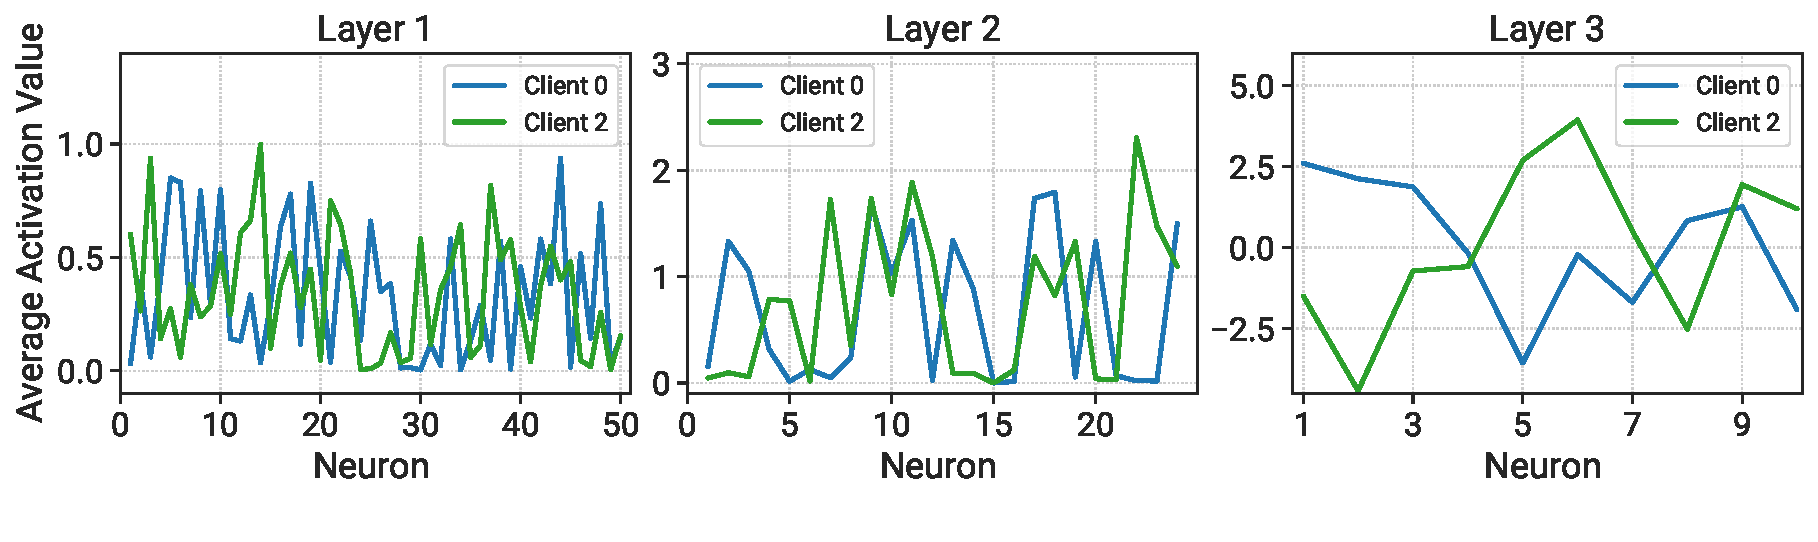
\includegraphics[width=0.95\linewidth]{chapter3/client0-2.pdf}
        % \caption{Client0与Client2每层神经元激活值对比}
        \label{fig:3-1client0-2}
    \end{subfigure}
    
    \vspace{0.3cm} % 调整子图之间的垂直间距
    
    \begin{subfigure}[b]{\textwidth}
        \centering
        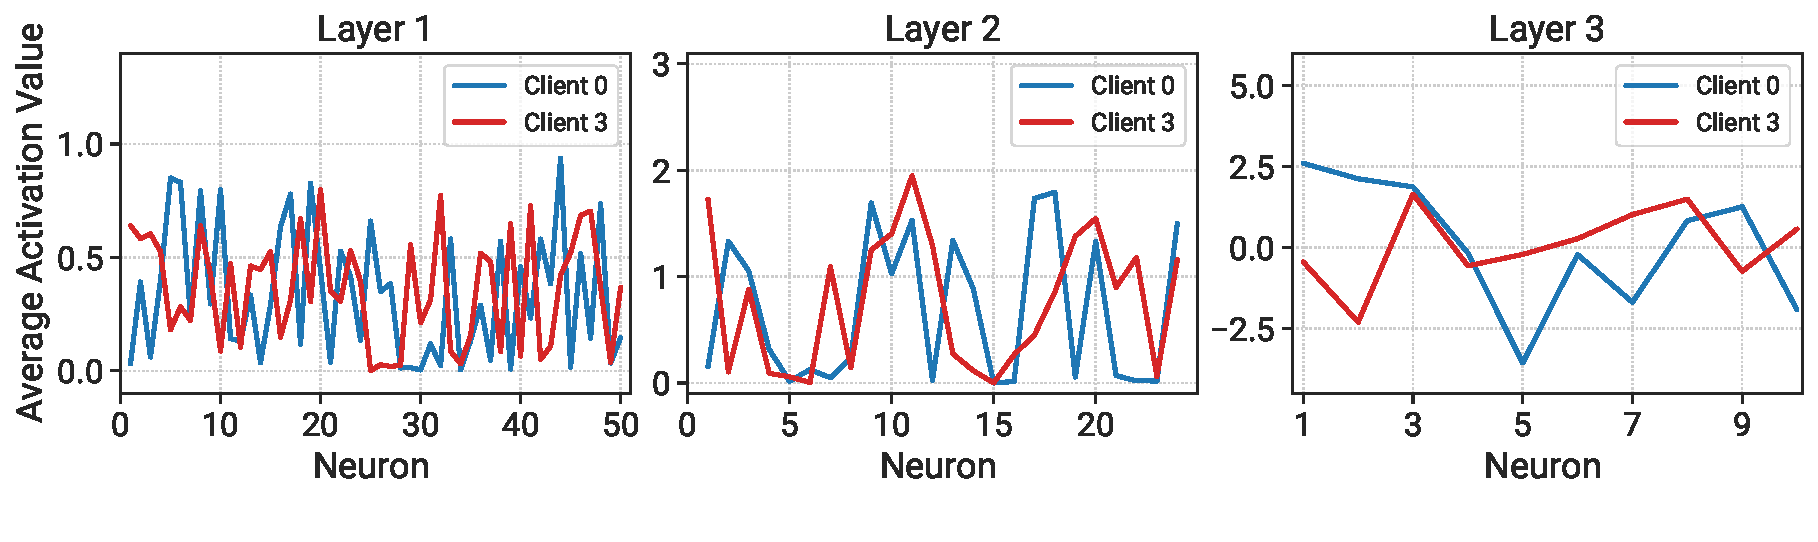
\includegraphics[width=0.95\linewidth]{chapter3/client0-3.pdf}
        % \caption{Client0与Client3每层神经元激活值对比}
        \label{fig:3-1client0-3}
    \end{subfigure}

    \vspace{0.3cm} % 调整子图之间的垂直间距
    
    \begin{subfigure}[b]{\textwidth}
        \centering
        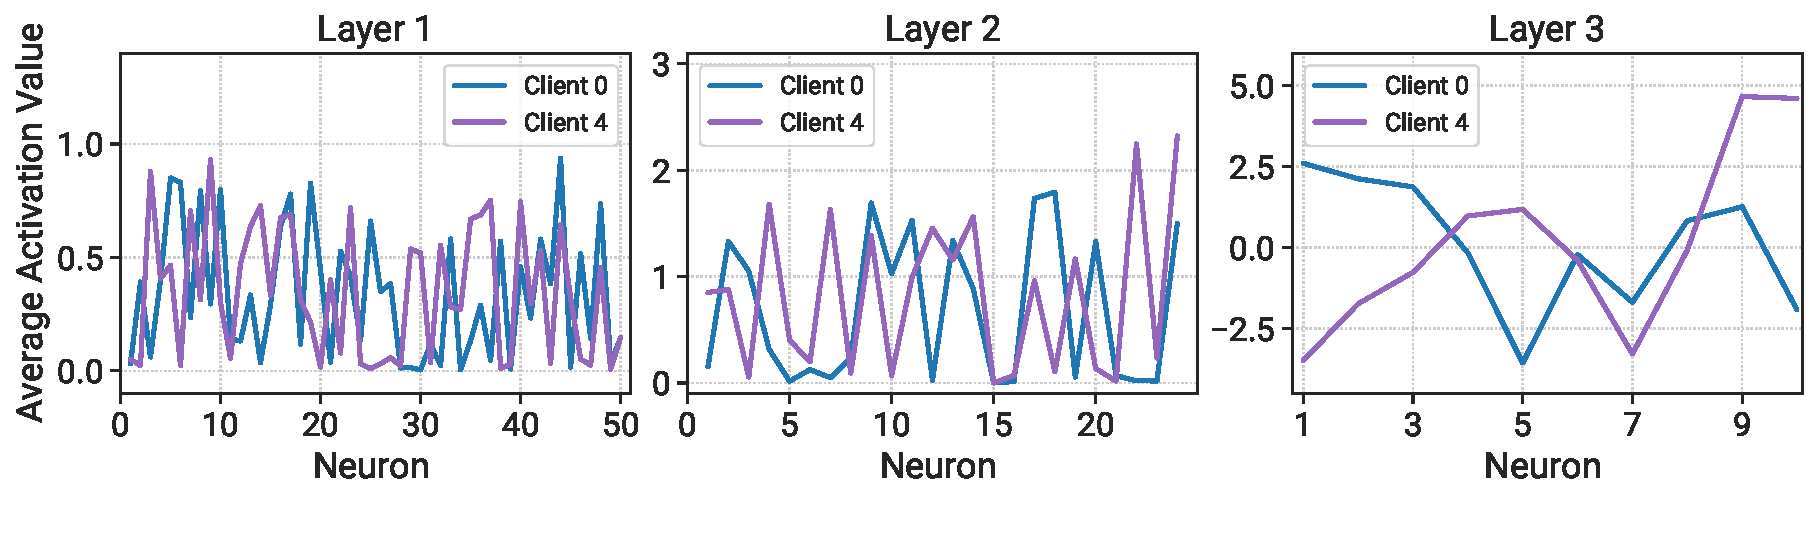
\includegraphics[width=0.95\linewidth]{chapter3/client0-4.pdf}
        % \caption{Client0与Client4每层神经元激活值对比}
        \label{fig:3-1client0-4}
    \end{subfigure}
    
    \vspace{0.3cm} % 调整子图之间的垂直间距
    
    \begin{subfigure}[b]{\textwidth}
        \centering
        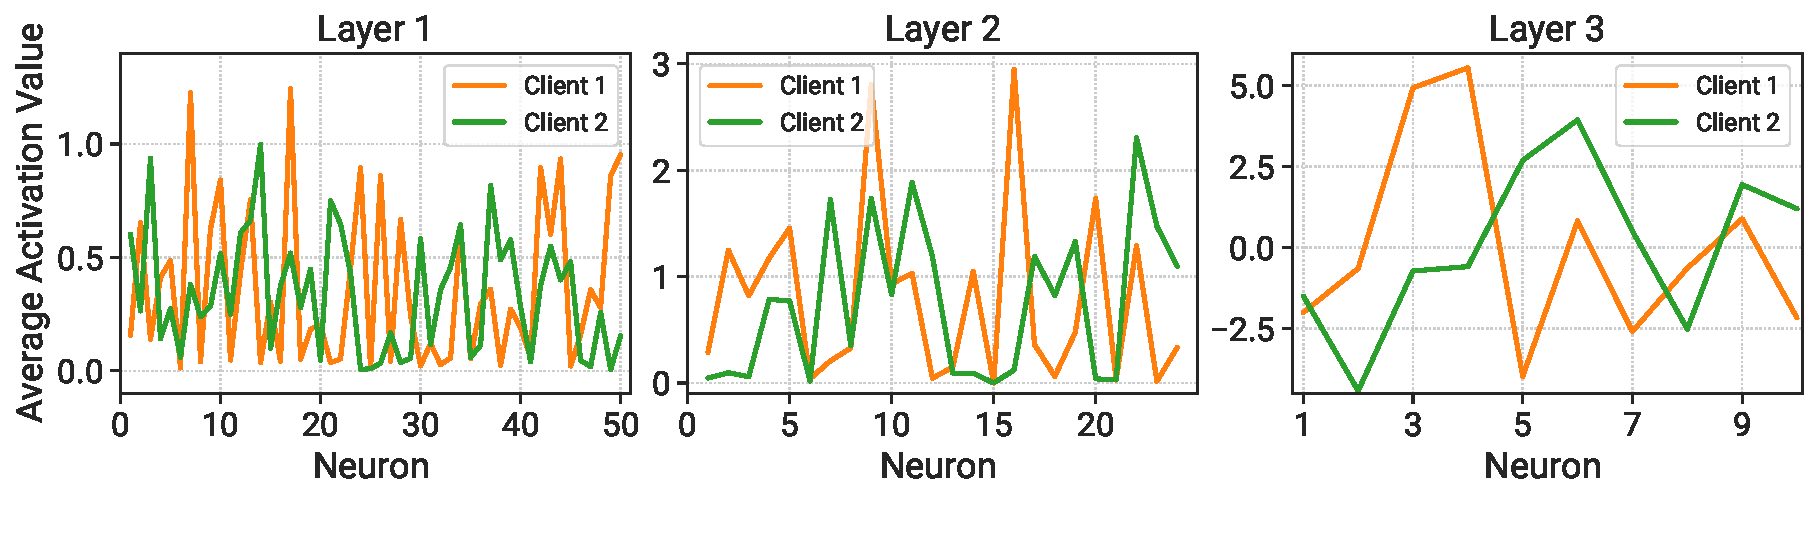
\includegraphics[width=0.95\linewidth]{chapter3/client1-2.pdf}
        % \caption{Client1与Client2每层神经元激活值对比}
        \label{fig:3-1client1-2}
    \end{subfigure}

    \vspace{0.2cm}
    \caption{Client0、Client1、Client2、Client3与Client4每层神经元激活值对比1}
    \label{fig:compare-clients0}
\end{figure}   

\begin{figure}[thbp]  
    \centering  
    \begin{subfigure}[b]{\textwidth}
        \centering
        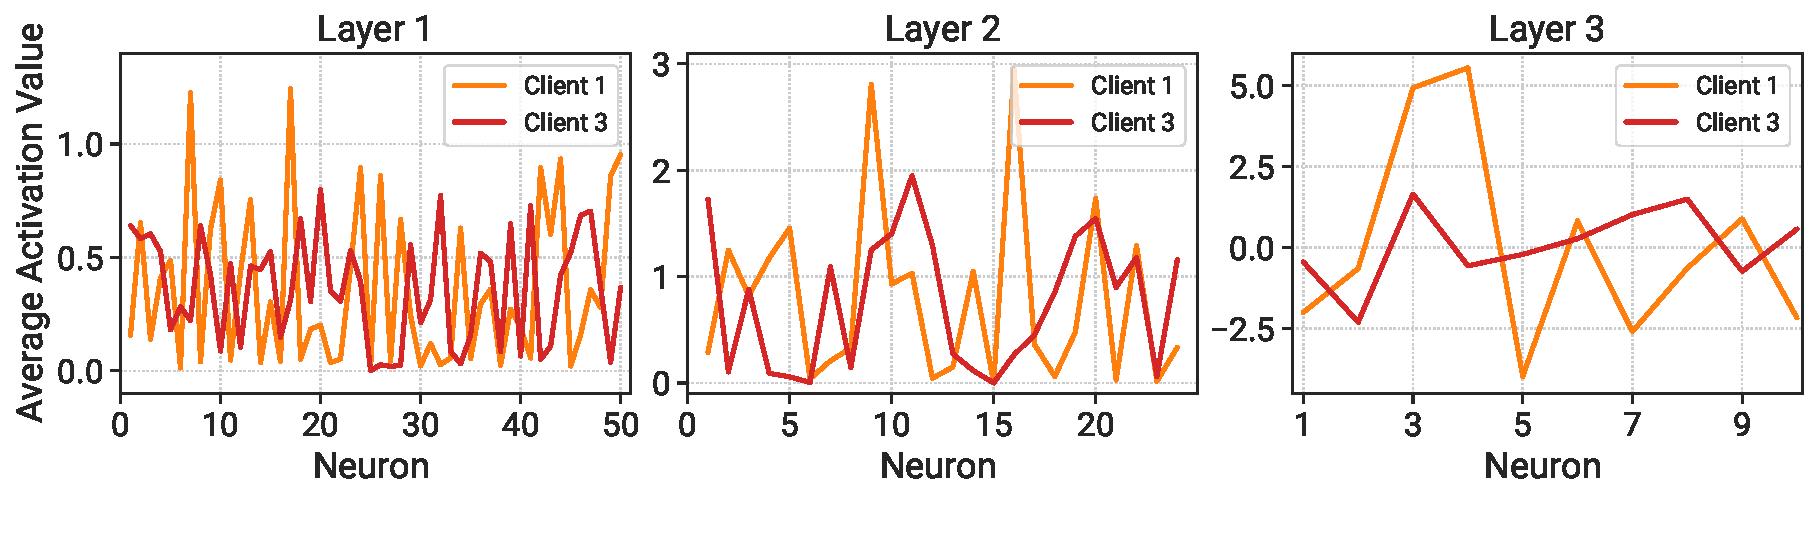
\includegraphics[width=0.95\linewidth]{chapter3/client1-3.pdf}
        % \caption{Client1与Client3每层神经元激活值对比}
        \label{fig:3-1client1-3}
    \end{subfigure}

    \vspace{0.3cm} % 调整子图之间的垂直间距
    
    \begin{subfigure}[b]{\textwidth}
        \centering
        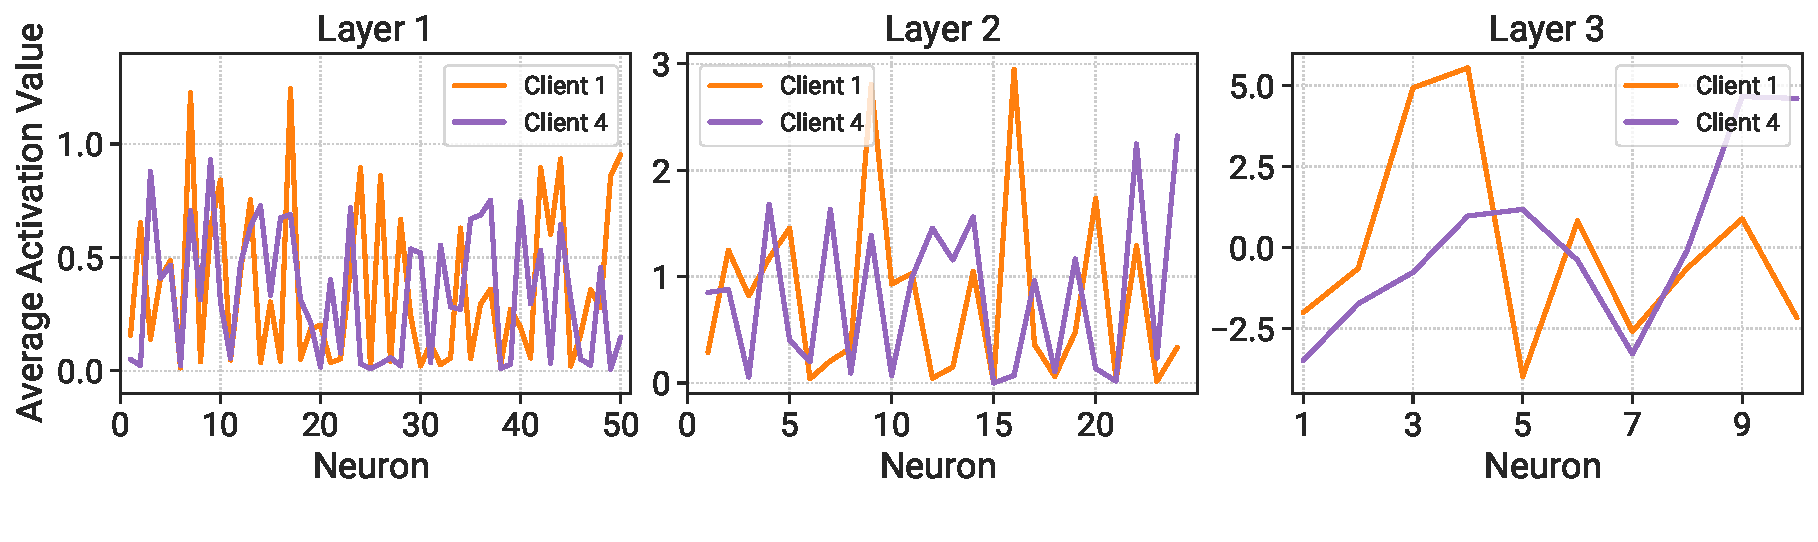
\includegraphics[width=0.95\linewidth]{chapter3/client1-4.pdf}
        % \caption{Client1与Client4每层神经元激活值对比}
        \label{fig:3-1client1-4}
    \end{subfigure}
    
    \vspace{0.3cm} % 调整子图之间的垂直间距
    
    \begin{subfigure}[b]{\textwidth}
        \centering
        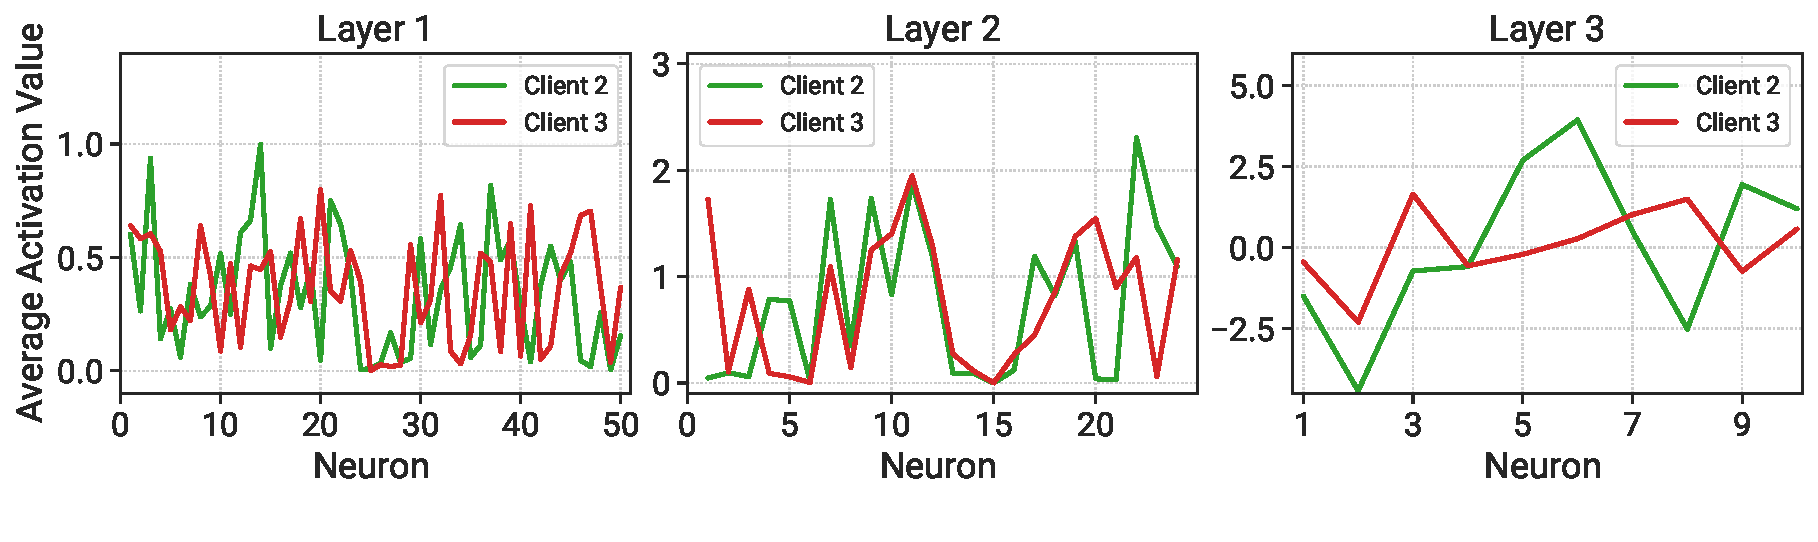
\includegraphics[width=0.95\linewidth]{chapter3/client2-3.pdf}
        % \caption{Client2与Client3每层神经元激活值对比}
        \label{fig:3-1client2-3}
    \end{subfigure}
    
    \vspace{0.3cm} % 调整子图之间的垂直间距
    
    \begin{subfigure}[b]{\textwidth}
        \centering
        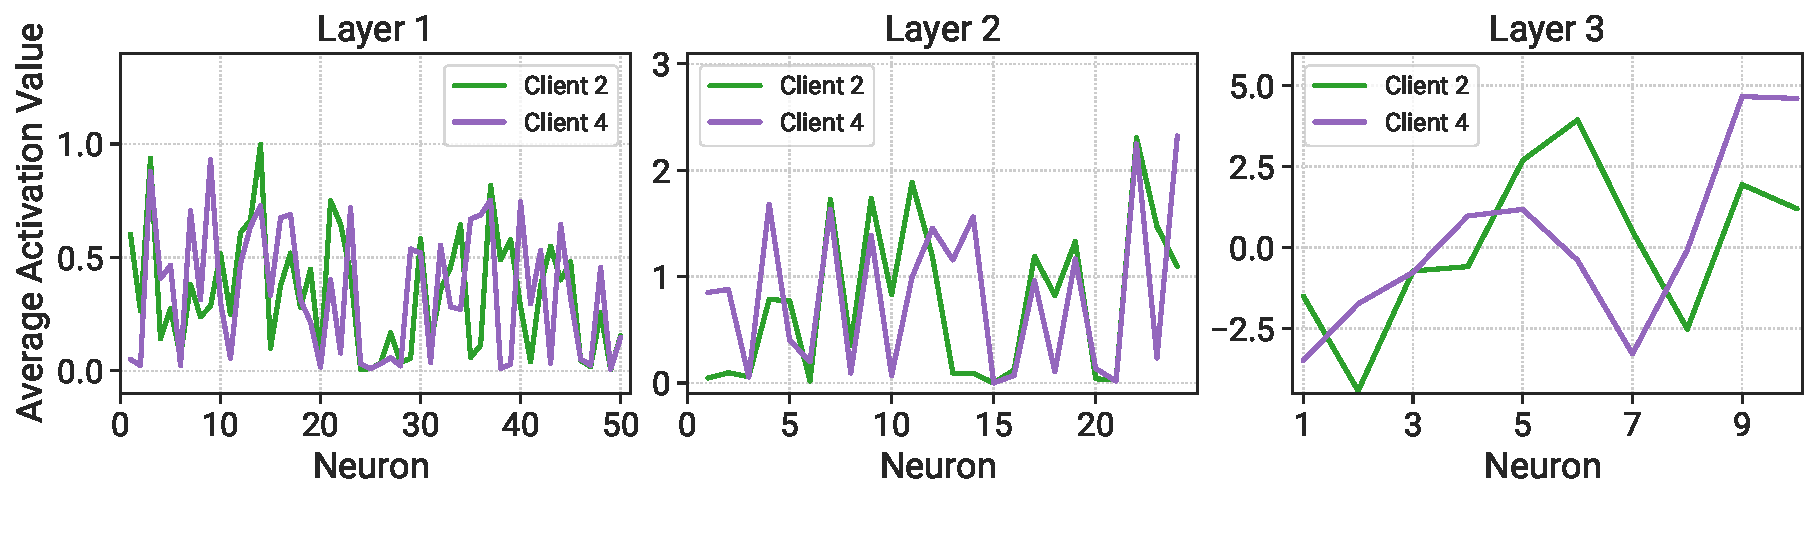
\includegraphics[width=0.95\linewidth]{chapter3/client2-4.pdf}
        % \caption{Client2与Client4每层神经元激活值对比}
        \label{fig:3-1client2-4}
    \end{subfigure}
    
    \vspace{0.3cm} % 调整子图之间的垂直间距
    
    \begin{subfigure}[b]{\textwidth}
        \centering
        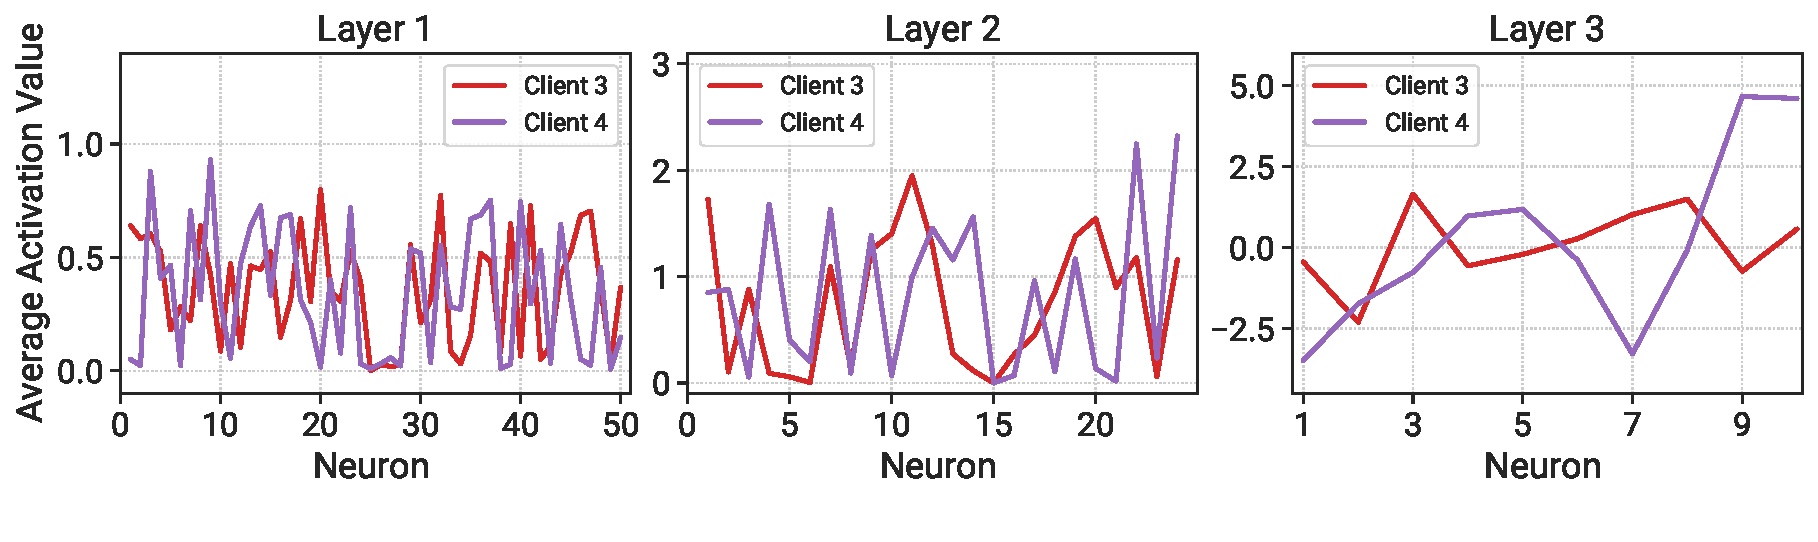
\includegraphics[width=0.95\linewidth]{chapter3/client3-4.pdf}
        % \caption{Client3与Client4每层神经元激活值对比}
        \label{fig:3-1client3-4}
    \end{subfigure}
    
    \vspace{0.2cm}
    \caption{Client0、Client1、Client2、Client3与Client4每层神经元激活值对比2}
    \label{fig:compare-clients1}
\end{figure}
%ppppppppppppppppppppppppppppppppppppp

\subsection{启发}
受这一发现的启发,我们提出了一种简单但有效的方法——FedDSE,
通过基于每个客户端的数据分布提取子模型来减少客户端之间的冲突。
本方法的主要思想是让每个客户端根据其本地数据集上的激活情况自适应地从整个模型中提取神经元,
其中选择激活幅度最大的神经元。
通过这种方式,冲突可以最小化,因为每个客户端都被分配了最适合其数据分布的神经元,
而不是那些被其他具有不同分布的客户端激活的神经元。
在不同数据集和模型上的实验结果表明,在资源受限的约束下,
相比基线方法可以显著提高训练效率。
我们的贡献如下:
\begin{itemize}
    \item 本文考虑了联邦学习(FL)中的数据异质性,
    并基于子模型提取进行了研究。我们的研究发现,
    具有不同数据分布的客户端往往会激活不同的神经元,
    如果神经元分配不当,会导致它们之间的冲突。

    \item 我们提出了一种新颖的训练方法FedDSE,
    根据每个客户端的数据分布为其提取子模型。
    在FedDSE 中,子模型的神经元是根据它们在每个客户端
    本地数据集上的激活水平选择的,
    从而能够为每个客户端分配最合适的神经元。
    
    \item 为了验证所提出方法的效率,FedDSE在与最新方法比较中取得最优。

\end{itemize}

\section{算法设计}
% 上述两个小章节介绍了以前方法引起的神经元冲突的问题,
% % 通过预实验分析了各个神经元激活值的分布,
% 观察到了不同边缘设备不同的神经元激活值分布以及
% 由此引起的神经元冲突现象。
% 对此提出了一种根据边缘设备数据分布自适应抽取神经元的方法
% FedDSE。
\subsection{符号设计}
我们考虑一个具有$L$层的深度神经网络,
第$l$层包含$m_l$个神经元,
我们将模型的权重参数表示为$\mathbf{w}$,
将第$l$层的参数表示为$\mathbf{w}_{l}=[w_l, b_l]$,
其中$w_l$和$b_l$分别是权重和偏置。
对于第 $l$ 层的第$i$个神经元,
我们计算其激活输出为
$h_{l,i} = \sigma (w_{l,i} \mathbf{h}_{l-1} + b_{l,i}) $,
其中 $\sigma(\cdot)$ 是非线性激活函数(例如 ReLU),
$w_{l,i}$ 和 $b_{l,i}$ 表示该神经元的权重和偏置,
$\mathbf{h}_{l-1}$ 表示前一层所有神经元的输出,
即 $\mathbf{h}_{l-1} = [h_{l-1,1},\ldots, h_{l-1,m_{l-1}}]$,
在二维的卷积神经网络中,
$h_l$代表一个二维的特征图。
为简单起见,我们将网络的所有权重表示为
$\mathbf{w}= [\mathbf{w}_1, \ldots, \mathbf{w}_L]$。
我们假设有 $N$ 个客户端,
每个客户端 $n$ 只能访问其自己的私有数据集 $\mathbb{D}_n:=\{x_i^n, y_i\}$,
其中 $x_i$ 表示第 $i$ 个输入数据样本,
$y_i \in \mathcal{C}=\{1,2,\cdots,C\}$ 表示 $x_i$ 对应的标签。
数据集 $\mathbb{D}_n$ 中的数据样本数量用 $D_n$ 表示。
$\mathbb{D}=\{\mathbb{D}_1, \mathbb{D}_2,\cdots,\mathbb{D}_N\}$,
其中 $N=\sum_{n=1}^{N}D_n$。
我们的目标是通过最小化整个数据集$\mathbb{D}$
上的损失来训练一个全局模型$\mathbf{w}$、
目标是优化公式\ref{equ:total_fl}与公式\ref{equ:total_fl_ap}。

\subsection{算法总体设计}
受到上述发现的启发,我们提出根据每个客户端的数据分布提取一个子模型,
详细的流程在算法\ref{alg:feddse}中展示。
我们的方法FedDSE具有以下创新点。
首先,考虑到充足的下载带宽,
我们允许每个客户端 $n$ 从服务器拉取整个模型 $\mathbf{w}$。
其次,基于神经网络的基本特性,即推理消耗的内存远少于训练,
每个客户端 $n$ 仅通过在部分本地数据集上推理来选择神经元。
最后,基于不同层的神经元激活幅度差异很大的观察结果,
每个客户端以逐层的方式提取神经元,这不需要缓存前一层神经元的激活值。
%ppppppppppppppppppppppppppppppppppppppp
\begin{figure}[thbp]
    \centering
    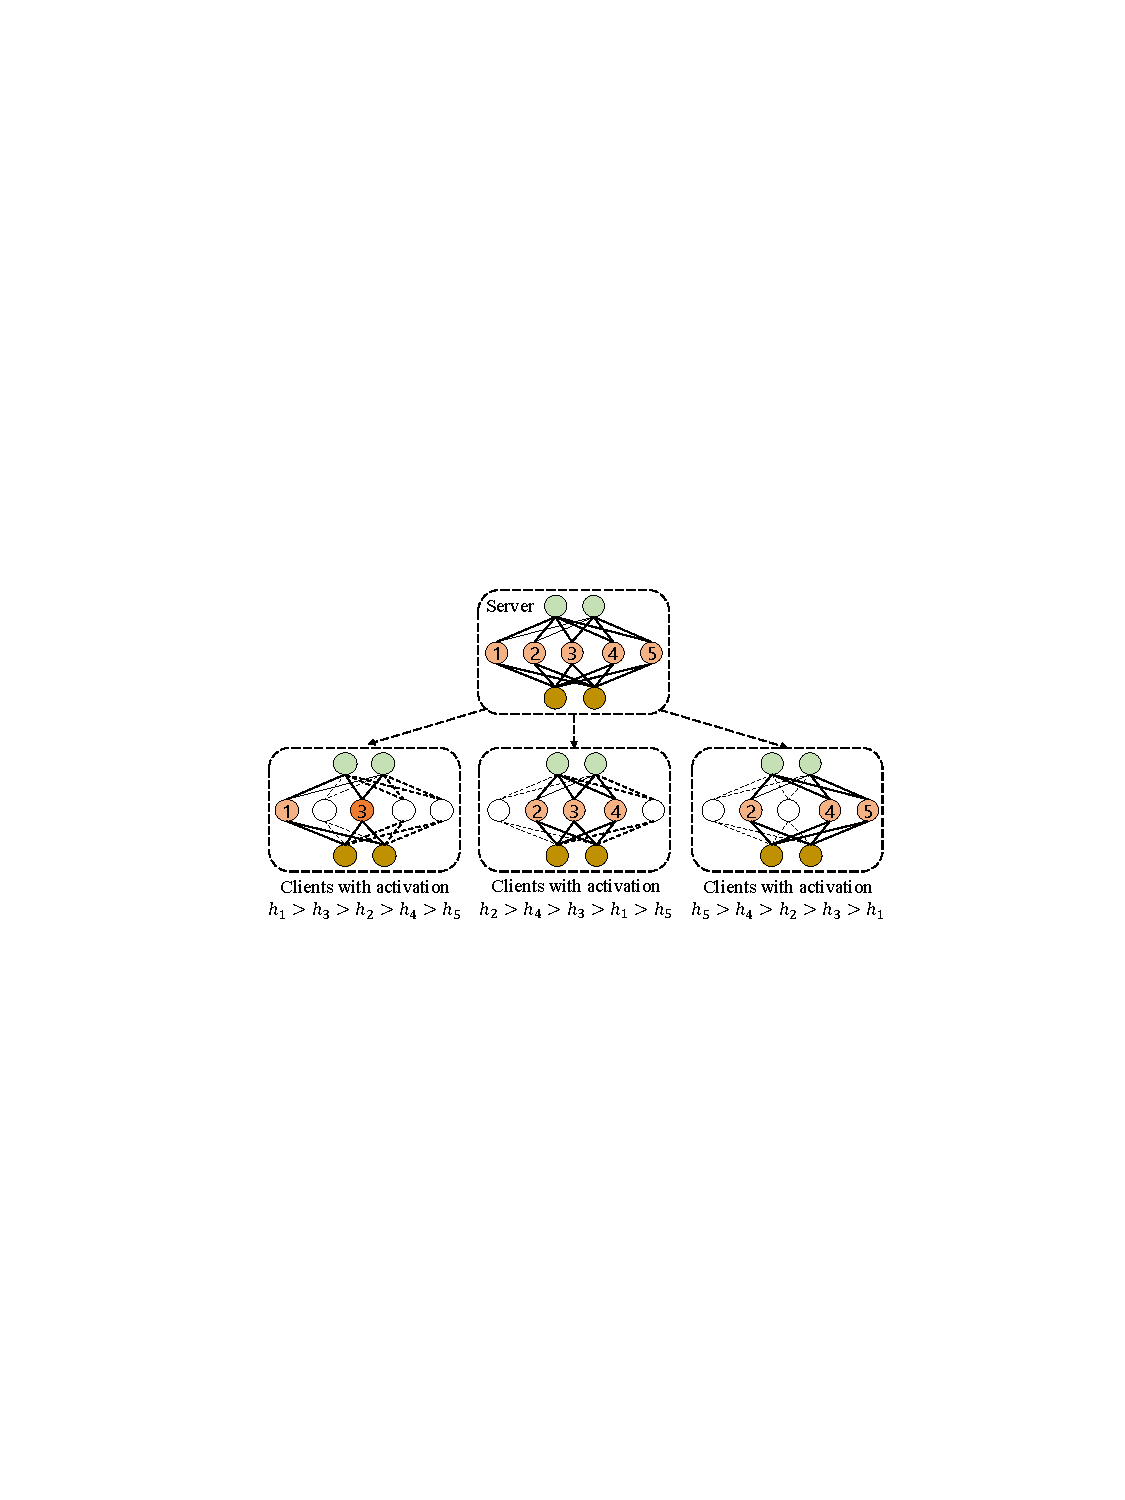
\includegraphics[width=0.9\linewidth]{chapter3/FedDSE.pdf}
    \caption{\label{fig:3-3-feddse}FedDSE方法抽取子模型}
\end{figure}
%ppppppppppppppppppppppppppppppppppppppp
如算法\ref{alg:feddse}所示,
首先在服务器端初始化全局模型,
然后再每一个轮次$t$中按照固定比例从所有的客户端中挑选出
子集$\mathcal{N}_t$参与本轮次训练。
服务器向挑选到的客户端发送全局模型参数,
然后客户端在自己的数据上训练模型。
唯一不同的是,在传统的FedAvg中,
客户端训练的是整个全局模型,
而在资源受限场景下,客户端训练的是全局模型抽取后的子模型。

FedDSE的核心算法部分就在于从全局模型抽取子模型的方法,
具体来说,对于每一层 $l$,客户端 $n$ 仅保留前 $r$ 比例的神经元
(以加权采样的方式),
并裁剪其他神经元以获得子模型,
通过如下公式获得:
\begin{equation}
    \mathbf{w}^n = \mathbf{w} \odot \mathbf{M}^n
\end{equation}
其中 $\odot$ 表示逐元素乘法,$\mathbf{M}^n$ 是掩码。
如果参数 $w_{l,i}$ 的神经元 $h_{l,i}$ 被裁剪,
则 $\mathbf{M}^n_{l,i}=0$,否则 $\mathbf{M}^n_{l,i}=1$。
每个神经元的采样概率基于其激活值确定。
我们对每个神经元 $i$ 的激活 $h_i$ 应用 softmax 函数,
得到其采样概率,公式如下:
\begin{equation}
    \label{equ:selectp}
    p(i)=\frac{e^{h_i/T}}{\sum_{j=1}^me^{h_j/T}}
\end{equation}
其中 $T$ 是温度。
显然,激活值越大的神经元越有可能被采样。
如图\ref{fig:3-3-feddse}所示,
当服务器端将全局模型分发给客户端的时候,
最左边的客户端选择了编号为$1$和$3$的神经元,
而裁剪了编号为$2$、$4$以及$5$的神经元。
本客户端这一层的激活值的排序情况是
$h_1 > h_3 > h_2 > h_4 > h_5$,
根据公式\ref{equ:selectp}选择编号为$1$和$3$的概率大于
其他的神经元,
结果便如图所示。
图\ref{fig:3-3-feddse}中的后两个子图也是如上述方法得到的。
具体$\mathbf{M}^n$的计算过程参考算法\ref{alg:GetMaskFedDSE}。
特别地,当温度 $T\rightarrow \infty$ 时,神经元以均匀方式选择,
而当温度 $T\rightarrow 0$ 时,
神经元以 Top-K 方式选择,即选择激活值最高的神经元 $\|h_{l,i}\|$。

当客户端抽取好本地的子模型之后,
按照下面的公式在本地数据上训练更新模型:
% 客户端在本地更新子模型按照下面公式:
\begin{equation}
    \mathbf{w}^n = \mathbf{w}^n - \eta \nabla_{\mathbf{w}^n} f_n(\mathbf{w}^n)
\end{equation}
其中 $f_n(\mathbf{w}^n)$ 表示数据小批量的损失,$\eta$ 是学习率。
然后,服务器接收所有客户端的子模型并聚合它们以更新全局模型:
\begin{equation}
    \mathbf{w} = \sum\nolimits_{n \in \mathcal{N}_t} \mathbf{P}_t^n \odot \mathbf{w}^n
\end{equation}
其中 $\mathcal{N}$ 表示选定的客户端集合,$\mathbf{p}^n$ 为每个子模型参数元素赋予权重。
我们设置:
\begin{equation}
    \mathbf{p}^n_{l,i}=\frac{1}{|\mathcal{N}_{l,i}|}
\end{equation}
其中 $\mathcal{N}_{l,i}$ 表示参与选择参数 $w_{l,i}$ 训练客户端集合里面数据数量。
最终经过$T$轮次的训练,
在服务器中心侧聚合出一个完整的符合要求的全局模型。
% 事实上,提取过程也可以通过使用无数据方式在服务器上进行。
%ccccccccccccccccccccccccccccccccccccccccccccccccccccccccccccccc
\begin{algorithm}[thbp]
    \caption{GetMaskFedDSE}
    \label{alg:GetMaskFedDSE}
    \begin{algorithmic}[1]
    \Require 客户端$n$的计算能力系数$r$,本地数据集$\mathbb{D}=\{ \mathbf{x}, \mathbf{y} \}$, $t$轮的全局模型$\mathbf{w_{t}}$
    \Ensure 客户端$n$在$t$轮的掩码$\mathbf{M^{n,t}}$
    
    \Procedure{GetMask}{$r_n$, $\mathbb{D}^p_n$, $\mathbf{w_{t}}$}
        \State $\mathbf{h^n} = f(\mathbf{w_t}; \mathbf{x, \mathbf{y}})$
        \For{对于每层激活值 $l \in \{1, \cdots, L  \}$}
            % \State $\mathbf{M}_{sorted} \leftarrow \max\limits_{i=0}^{r_n \cdot I_l}g_{l,0}^n,g_{l,1}^n,\dots,g^n_{l,I_l-1}$ 
            \State $\mathbf{S}_{sorted} \leftarrow \textbf{sort}([h_{l,1},\ldots, h_{l,m_l}])$
            \State $\mathbf{S}_{top-r} = \mathbf{S}_{sorted}[1 : r \cdot m_l]$
            \If{ $\mathbf{h_{l,i}} \in \mathbf{S}_{top-r}$}
              $\mathbf{M^{n,t}_{l,i}} = 1$
            \Else \text{ }$\mathbf{M^{n,t}_{l,i}} = 0$
            \EndIf
        \EndFor
        \State \Return $\mathbf{M^{n,t}}$
    \EndProcedure
\end{algorithmic}
\end{algorithm}
%ccccccccccccccccccccccccccccccccccccccccccccccccccccccccccccccc


%ccccccccccccccccccccccccccccccccccccccccccccccccccccccccccccccc
\begin{algorithm}[thbp]
    \caption{FedDSE}\label{alg:feddse}
    \begin{algorithmic}[1]
    \Require 全局模型参数$\mathbf{w}$,
                学习率 $\eta$,
                总通讯次数$T$,
                本地客户端训练次数$E$
    \Ensure $T$轮的全局模型参数$\mathbf{w}_{T+1}$
    \State 初始化全局模型参数$\mathbf{w}_1$
    \Procedure{Server-side Optimization}  {}
        \For {对每个轮次$t \in \{1, \cdots, T \}$}
            \State 随机挑选所有客户端的子集$\mathcal{N}_t$
            \For {对于每个挑选到的客户端$n$\textbf{并行执行}}
                \State $\mathbf{w}_{t+1}^n \leftarrow \textbf{ClientLocalUpdata}(\mathbf{w}_t)$
            \EndFor
            \State 更新全局模型参数
            $\mathbf{w}_{t+1} = 
            \sum\nolimits_{n \in \mathcal{N}_t} \mathbf{P}_t^n 
            \odot \mathbf{w}_t^n $
        \EndFor
    \EndProcedure

    \Procedure{ClientLocalUpdate}{$\mathbf{w}_t$}
        \State 从服务器侧接收$\mathbf{w}_t$
        \State $\mathbf{M}_t^n \leftarrow \textbf{GetMask}(\mathbf{w}_t)$
        \State 初始化$\mathbf{w^n_{t,0}} = \mathbf{w}_t \odot \mathbf{M}_t^n$
        \For{从$1$到$E$迭代轮次$e$}
            \State 更新本地模型
            $\mathbf{w^n_{t,e+1}} = \mathbf{w^n_{t,e}} - \eta \nabla_{\mathbf{w^n_{t,e}}} f_n(\mathbf{w^n_{t,e}})$
        \EndFor
        \State \Return $\mathbf{w^n_{t,E+1}}$
    \EndProcedure
\end{algorithmic}
\end{algorithm}
%ccccccccccccccccccccccccccccccccccccccccccccccccccccccccccccccc


\section{实验过程与结果分析}
\label{sec:feddseexp}
为了验证我们的方法的高效性与准确性,
我们选择了基于卷积神经网络的图片分类实验,
这也是大多数联邦学习论文所用到的实验。
\subsection{数据集与模型选择}
\label{sec:feddsedata_model}
我们在三个模型和四个主流数据集上评估了所提出的FedDSE的性能,
包括用于EMNIST\cite{lecun1998mnist}的简单的卷积神经网络,
用于CIFAR-10和CIFAR-100\cite{krizhevsky2009learning}的ResNet18\cite{shafiq2022deep},
以及用于TinyImageNet\cite{le2015tiny}的ResNet34。
与HeteroFL\cite{diao2020heterofl}类似,
我们采用了静态批量归一化,
并在每个卷积层之后使用了一个标量模块。
简单的卷积神经网络的通道数分别为$\{ 64, 128, 256, 512 \}$,
具体的结构如图\ref{fig:2-2-2-conv}所示。
而模型ResNet18与ResNet34则与表\ref{tab:resnet}中的架构一致。
数据集方面我们使用了四个数据集,
分别是EMNIST、CIFAR-10、CIFAR-100以及TinyImageNet,
具体信息如表\ref{tab:datasets}所示,
从上到下数据量增加分类数量逐渐增加,
数据集难度有所提升。
\begin{table}[thbp]
    \caption{\label{tab:datasets}不同数据集信息}
    \begin{tabularx}{\linewidth}{l X<{\centering} X<{\centering} X<{\centering}}
        \toprule
        数据集名称 & 训练集(条) & 测试集(条) & 类别(类) \\ \hline
        EMNIST & $60000$ & $10000$ & $10$ \\ 
        CIFAR-10 & $50000$ & $10000$ & $10$ \\ 
        CIFAR-100 & $50000$ & $10000$ & $100$ \\ 
        TinyImageNet & $100000$ & $10000$ & $200$ \\ 
        \bottomrule
    \end{tabularx}
\end{table}
\subsection{实验设置}
\textbf{数据异质性 } 
为了模拟现实情况中的数据异质性的特征,
我们遵循HeteroFL中的设定方法\cite{li2020federated, diao2020heterofl},
给不同的客户分配固定的数据种类,
就是不同的客户中仅仅包含我们设定分配种类的数据,
而不会包含其他种类的数据,
以此来模拟现实中的中的非独立同分布(non-IID)特性。
根据每位客户分配种类的数量,
我们将设定两种情况,
分别是\textbf{高数据异质性}和\textbf{低数据异质性},
顾名思义,
高数据异质性客户端分配到的数据种类更少,
也就意味着数据更具体本地特色,
与其他客户端数据分布差距更大;
那么,
低数据异质性设定中每个客户分配更多种类的数据,
也就是不同客户之间重复种类的数量增多,
数据的泛化性更好,
与其他客户端数据分布差别相较高数据一致性小。
我们根据不同的数据集来设定不同数据异质性所需要的种类数,
如表\ref{tab:classinfo}所示,
分别表示列出了四个数据集高低数据异质性的情况,
例如在EMNIST数据集,
高数据异质性给客户端分配的种类数是$2$种,
而低数据异质性分配则是$4$种。
\begin{table}[thbp]
    \caption{\label{tab:classinfo}不同数据集信息}
    \begin{tabularx}{\linewidth}{c X<{\centering} X<{\centering} X<{\centering} X<{\centering}}
        \toprule
        数据集 & EMNIST & CIFAR-10 & CIFAR-100 & TinyImageNet \\ \hline
        高数据异质性 & $2$ & $2$ & $8$ & $16$ \\ 
        低数据异质性 & $4$ & $4$ & $16$ & $32$ \\ 
        \bottomrule
    \end{tabularx}
\end{table}

\textbf{模型异质性 }
在模拟现实环境中的边缘设备的资源分布场景中,
FedDSE主要应用于低质量客户端分布场景,
指的是在所有的客户计算资源分布中不存在达到中心侧服务器水平的客户端,
意味着中心侧模型不会被任何一个客户端完整训练。
因此我们设定了五种不同客户端计算资源分别是
% $r = \{ 0.99, \frac{1}{2}, \frac{1}{4}, \frac{1}{8}, \frac{1}{16} \}$,
$\mathbf{r} = \{ 0.99, 0.5, 0.25, 0.125, 0.0625 \}$,
为了模拟低质量客户端分布\cite{li2020federated, diao2020heterofl},
本章实验我们设定最高的比例为$0.99$。
其中$r$中的$0.5$表示客户端资源能力有服务器端的$\frac{1}{2}$,
服务器端可以训练整个全局模型的所有神经元,
而$r=\frac{1}{2}$的客户端可以训练全局模型一半的神经元。
同时,我们设定上述中的五种设定都是均匀分布的,
也就是说每种分布都占客户端总数的百分之二十。

\textbf{baseline方法 }
我们比较了近期的四种比较主要的方法,
分别是HeteroFL、FedRolex、Federated Dropout以及DepthFL作为
FedDSE的对比方法。
为了保证比较的公平性,我们对所有方法使用了相同的学习率、本地训练轮数以及通信轮数。
每种数据集对应的具体训练参数见表\ref{tab:train_info}。
\begin{table}[thbp]
    \caption{\label{tab:train_info}不同数据集训练参数设置}
    \begin{tabularx}{\linewidth}{l X<{\centering} X<{\centering} X<{\centering} X<{\centering}}
        \toprule
        & EMNIST & CIFAR-10 & CIFAR-100 & TinyImageNet \\ \hline
        本地训练次数(E) & $2$ & $2$ & $2$ & $2$ \\ 
        学习率 & $0.001$ & $0.001$ & $0.001$ & $0.001$ \\ 
        训练轮次 & $800$ & $2500$ & $2500$ & $2500$ \\ 
        优化器 & SGD & SGD & SGD & SGD \\ 
        动量 & $0.9$ & $0.9$ & $0.9$ & $0.9$ \\ 
        权重衰减 & $5.00\text{E}-04$ & $5.00\text{E}-04$ & $5.00\text{E}-04$ & $5.00\text{E}-04$ \\ 
        推理数据数量 & 全部 & 全部 & 全部 & 全部 \\ 
        \bottomrule
    \end{tabularx}
\end{table}
其中简单数据集EMNIST的训练轮次是$800$,
其余的数据集的训练轮次都是$2500$。
数据中的推理数据数量是指每次抽取子模型时,
使用本地数据推理得到激活值过程中使用的数据数量,
本实验中用到了本地全部数据进行推理。
本地训练次数是指在客户端训练子模型的次数。
所有的训练过程使用的都是随机梯度下降(Stochastic Gradient Descent, SGD)优化器。

\textbf{训练配置以及平台 }
对于EMNIST、CIFAR-10、CIFAR-100以及TinyImageNet,
我们应用了边界框裁剪来增强图像\cite{zoph2020learning}。
在每个通讯轮次中从设定的$100$个客户端中选出百分之十进行训练,
$frc = 10\%$。
选定的客户的计算能力符合均匀分布。
实验在实验在PyTorch框架\cite{paszke2019pytorch}上进行,
本章实验设备是Nvidia 3090。

\textbf{评估指标 }
对于图像分类任务,我们采用全局准确率作为评估指标,
定义为服务器模型在整个测试集上的准确率。

\subsection{训练细节}
\label{sec:feddse_tricks}
\textbf{掩码交叉熵损失 }
已经证明,联邦学习( FL )的失败可以归因于在多次迭代中
局部训练的局部模型参数之间的权重差异。
这种权重差异主要体现在神经网络的最终分类层。
因此,与使用包含所有类的完全交叉熵损失不同,
每个局部模型的训练只与它们各自的类有关。
允许每个局部模型根据可用的局部标签信息专注于特定的子任务。
为了实现这一点,引入了掩码交叉熵损失,
它涉及在应用损失函数之前将模型的输出掩蔽掉。

\textbf{放缩模块 }
由于通过多个轮次优化客户端模型,
因此在不同计算复杂度水平下的局部模型的参数可能会出现偏差,
并在尺度上发生变化。
这种现象被称为偏移\cite{srivastava2014dropout}。
在推断阶段,为了直接利用全模型,采用了偏移率为q。
该技术在训练阶段对输入值进行$\frac{1}{1-q}$的缩放。
本文引入放缩模块,
插在参数层之后,
在激活层之前。
该缩放模块在训练阶段以的$\frac{1}{1-q}$因子对输入值进行缩放。
在全局聚合之后,保证全局模型可以直接使用。

\textbf{静态批归一化 }
批归一化\cite{NEURIPS2018_36072923,andreux2020siloed}( Batch Normalization, BN )在深度学习模型中被广泛使用。
然而,许多主流算法避开了BN。
与BN相关的一个重要问题是需要对每个隐藏层的表示进行连续估计。
将这些统计数据传递给服务器的过程会导致通信成本增加,并引发隐私担忧。
静态批归一化(static Batch Normalization, sBN)被应用于优化隐私受限的异构模型。
在训练阶段,sBN只是简单地对批量数据进行归一化处理,并没有对运行估计值进行跟踪。
因为每个通信轮都是独立的,sBN适用,
在完成训练过程后,服务器依次查询本地客户端。

\subsection{实验结果}
表\ref{tab:total_high_res}和表\ref{tab:total_low_res}分别展示了我们的方法
与上述四个基线方法在高数据异质和低数据异质性情况下的对比结果。
FedDSE的温度设置为0。
五个方法全部从EMNIST到TinyImagenet准确率都是逐渐下降的,
而且在EMNIST数据集上所有方法准确率可以达到百分之九十往上,
而在数据集TinyImagenet上仅仅只能达到百分之十五左右。
由此我们将EMNIST分为简单数据集,
将CIFAR-10设定为中等数据集,
而将CIFAR-100和TinyImagenet认定为困难数据集。

\begin{table}[thbp]
    \caption{\label{tab:total_high_res}低质量客户端分布场景中在高数据异质性下不同方法准确率对比}
    \begin{tabularx}{\linewidth}{l X<{\centering} X<{\centering} X<{\centering} X<{\centering}}
        \toprule
        方法 & EMNIST & CIFAR-10 & CIFAR-100 & TinyImageNet \\ \hline
        HeteroFL & $93.21$ & $38.13$ & $8.00$ & $5.72$ \\ 
        Federated Dropout & $87.96$ & $50.16$ & $10.47$ & $10.17$ \\ 
        FedRolex & $91.41$ & $55.61$ & $14.02$ & $15.39$ \\ 
        DepthFL & $92.34$ & $49.42$ & $11.22$ & $12.45$ \\ 
        FedDSE & \textbf{95.34} & \textbf{58.19} & \textbf{16.61} & \textbf{22.19} \\ 
        \bottomrule
    \end{tabularx}
\end{table}
表\ref{tab:total_high_res}也就是在高数据异质情况下,
FedDSE在所有的数据集中取得了最好的准确率。
相对于其余四个方法中最好的分别提高了
$2.13\%$、$2.58 \%$、$2.59 \%$和$6.80\%$。
对简单数据集和中等数据集的提升大多数在百分之二左右,
而对于困难数据集TinyImagenet的提升有百分之六点八之多。
可以看出,
FedDSE相较于其他四个方法都是准确率更高,
特别是在困难数据集上的提升更为显著。
这表明,当类别数量相对较少时,
我们的方法能够准确捕捉并激活相关神经元进行训练,
使得FedDSE方法显著好于其他方法。
整体来看,
Federated Dropout于其他方法相比表现的最差,
这也与方法中随机选择神经元有很大的关系;
HeteroFL在简单数据集上表现稳定,
但是对于中等和困难数据集准确率出现了灾难性下滑,
由于其在中等与困难数据集上有神经元未参与训练造成的;
FedRolex是除了我们方法之外最优的方法,
对于所有等级数据集表现稳定且准确率较高;
DepthFL表现稳定但效果一般。
\begin{table}[thbp]
    \caption{\label{tab:total_low_res}低质量客户端分布场景中低数据异质性下不同方法准确率对比}
    \begin{tabularx}{\linewidth}{l X<{\centering} X<{\centering} X<{\centering} X<{\centering}}
        \toprule
        方法 & EMNIST & CIFAR-10 & CIFAR-100 & TinyImageNet \\ \hline
        HeteroFL & $97.61$ & $47.01$ & $11.16$ & $10.52$ \\ 
        Federated Dropout & $97.63$ & $58.16$ & $16.21$ & $19.18$ \\ 
        FedRolex & $98.61$ & $68.04$ & $20.81$ & $19.44$ \\ 
        DepthFL & $97.75$ & $55.93$ & $17.87$ & $20.99$ \\ 
        FedDSE & \textbf{98.65} & \textbf{70.82} & \textbf{22.93} & \textbf{22.88} \\ 
        \bottomrule
    \end{tabularx}
\end{table}

表\ref{tab:total_low_res}是在低数据异质情况下五个方法的对比情况。
FedDSE是所有方法中准确率最高的,
相对于其余四个方法中最好的分别提高了
$0.04\%$、$2.78 \%$、$2.12 \%$和$1.87\%$。
在低数据异质这种简单的情况下,
在EMNIST上所有方法的差距缩小,
而在中等和困难数据集上不同方法的差距也仅有百分之二左右。
% HeteroFL方法在简单场景下表现效果不佳
FedRolex方法是除了我们方法之外表现最好的,
HeteroFL方法在简单场景下表现不佳,与存在未参与训练神经元有关。
总体来说在简单场景下,
所有所有方法的差距在缩小,
因为低数据异质情况下各个客户端数据分布更加相似导致
联邦学习的训练难度下降。

%ppppppppppppppppppppppppppppppppppppppp
\begin{figure}[thbp]
    \centering
    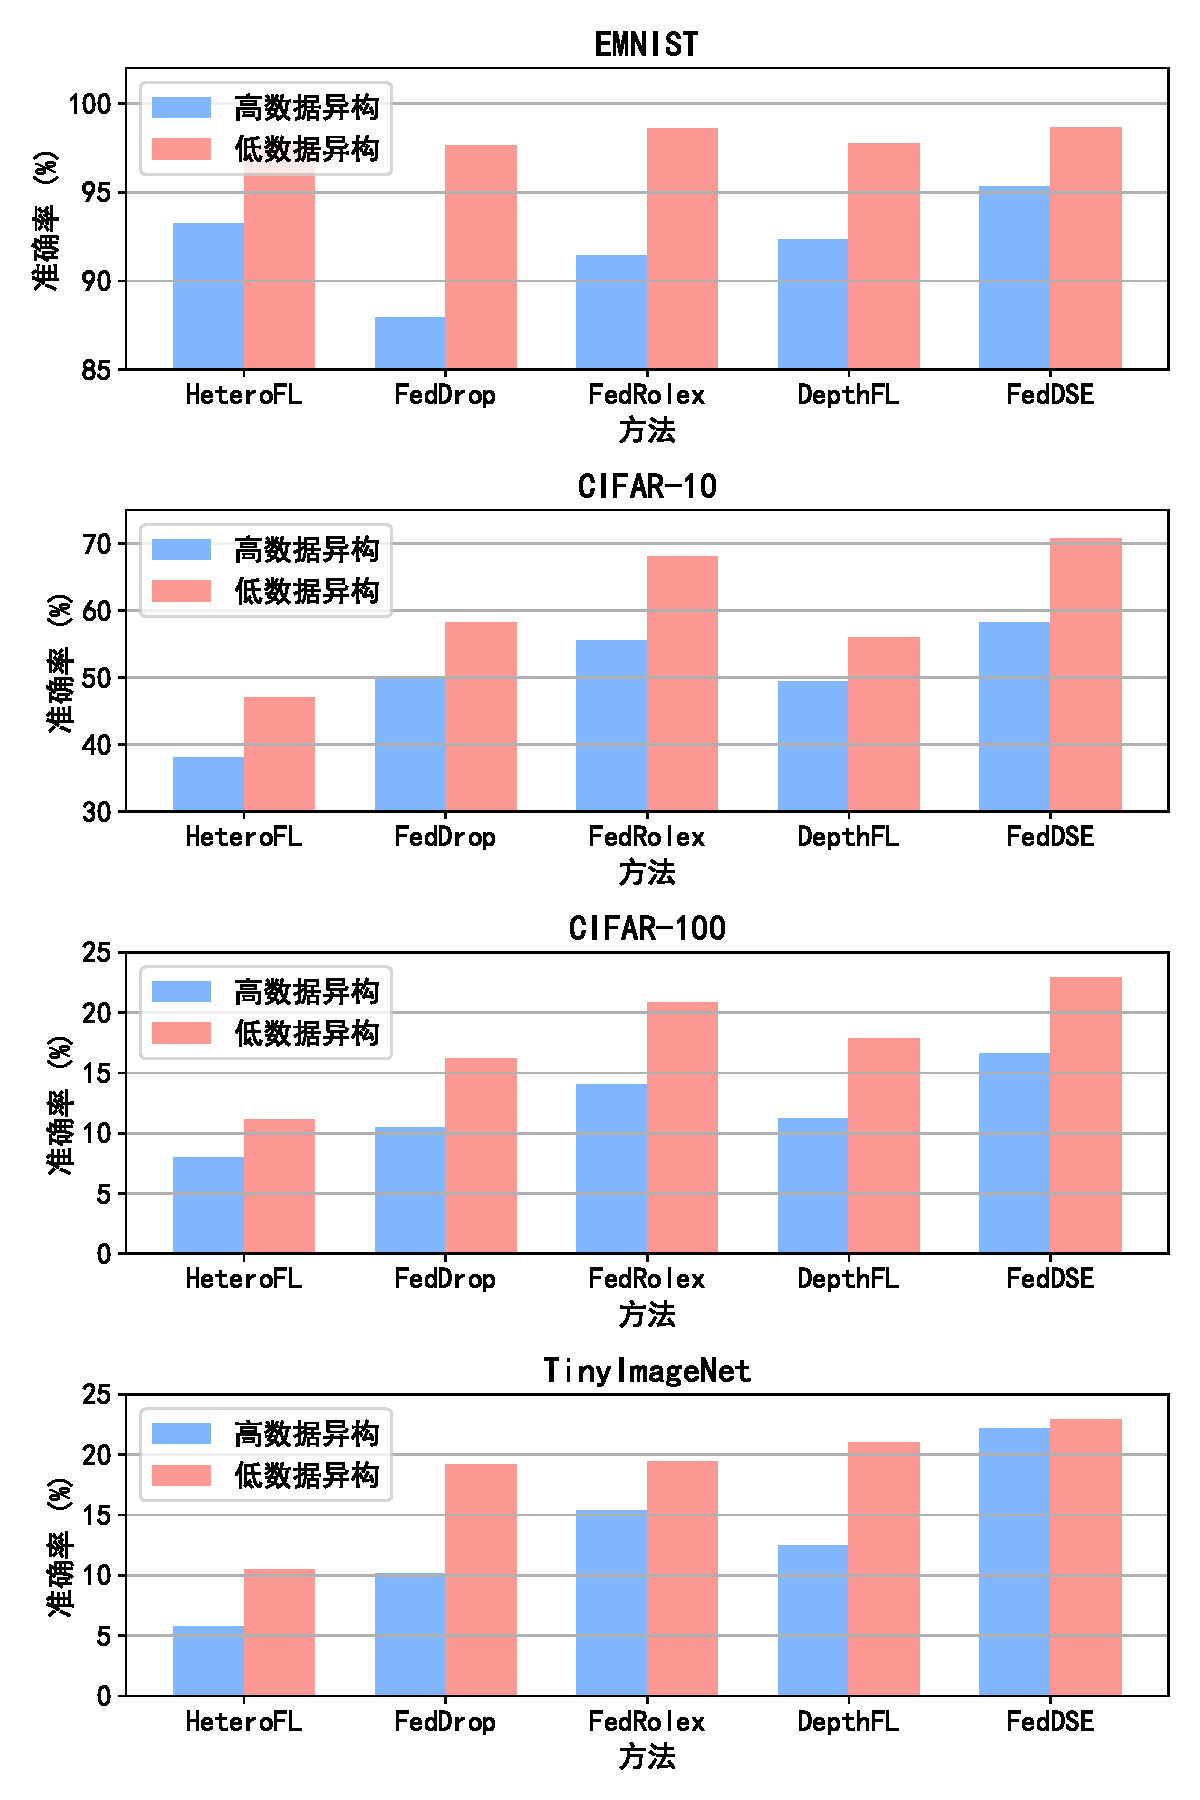
\includegraphics[width=0.95\linewidth]{chapter3/compare_res1.pdf}
    \caption{\label{fig:3-3-compare_res}高低数据异质性对比图}
\end{figure}
%ppppppppppppppppppppppppppppppppppppppp
图\ref{fig:3-3-compare_res}描述了五个方法在不同数据集上的
对应高数据异质性与低数据异质性的准确率。
非常直观的我们可以观察到高数据异质性的准确率远远低于
低数据异质性的准确率,
这是因为在低数据异质性条件下,
客户端数据集均匀分布,模型收敛更快,
显著减少了训练开销。
其中,
Federated Dropout方法高低数据异质性在不同数据集中对准确率的影响较大,
而HeteroFL、FedRolex与DepthFL则在所有数据集中高低数据集影响较为稳定。
FedDSE在最高难度的数据集上TinyImagenet上,
高低数据集对准确率的印象较小,
两者差距很接近,
这意味着我们的方法在困难数据集和高数据异质情况下会取得较好的效果,
达到了与低数据异质性相同的准确率。

\section{消融实验}
\subsection{客户端计算能力分布对模型能力的影响}
在上述实验中,客户端容量的分布是均匀设置的,
就是每个计算能力客户端的占比都是百分之二十。
为了观察不同的客户端占比对最终结果的影响,
我们选择了两种客户端计算能力分别是
$\beta = \{ \frac{1}{2} , \frac{1}{16}  \}$。
然后我们定义$\rho$为计算能力为$\frac{1}{2}$的客户端
占总共客户端的比例,
例如$\rho = 0.8$表示计算能力为$\frac{1}{2}$的客户端
占到所有客户端的比例是$0.8$,
计算能力为$\frac{1}{16}$的占客户端总数的$0.2$。
最后$\frac{1}{2}$计算能力的用户占比从零到一
观察对准确率的影响,
我们在简单数据集EMNIST和中等数据集CIFAR10上进行了实验。

%ppppppppppppppppppppppppppppppppppppppp
\begin{figure}[thbp]
    \centering
    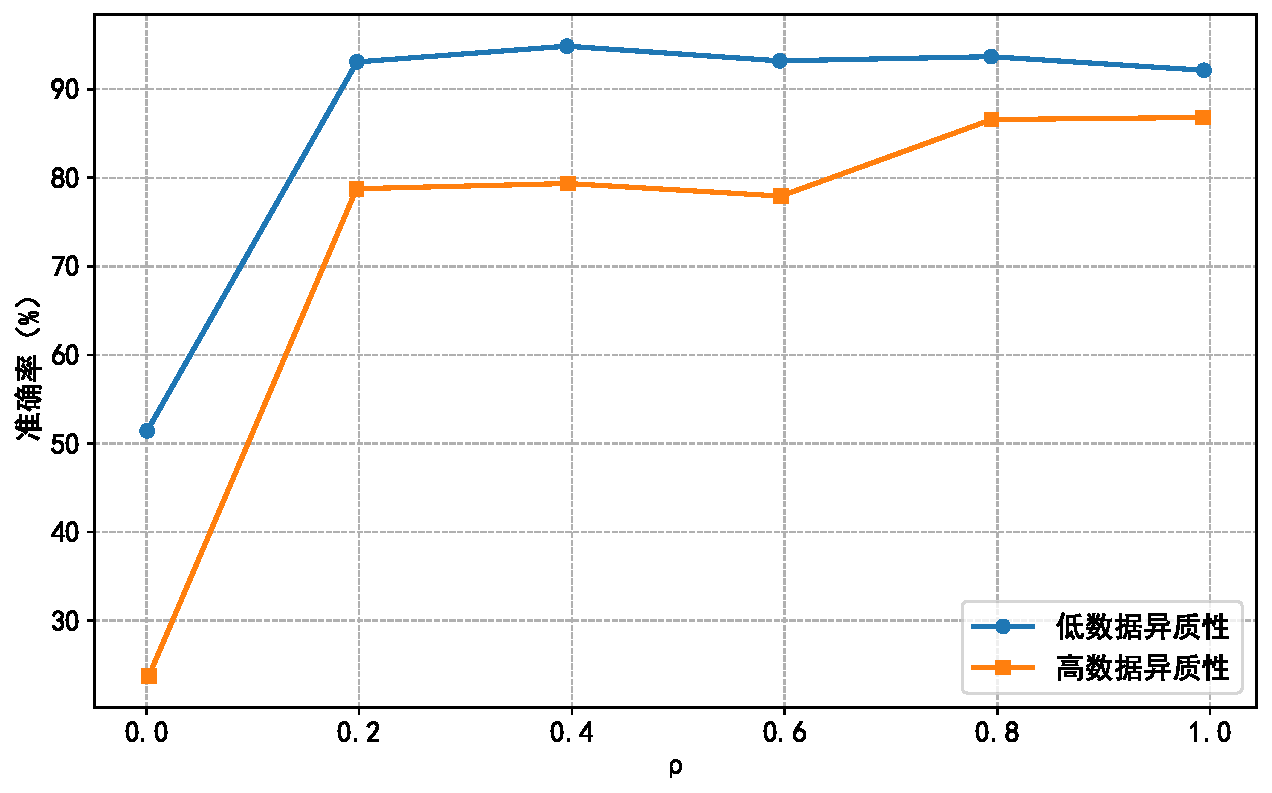
\includegraphics[width=0.9\linewidth]{chapter3/emnist_rou.pdf}
    \caption{\label{fig:3-4-emnist-rou}EMNIST上$\rho$对准确率影响曲线图}
\end{figure}
%ppppppppppppppppppppppppppppppppppppppp
在EMNIST上的结果如图\ref{fig:3-4-emnist-rou}所示,
我们可以观察到,
首先高数据异质性的准确率均比低数据异质性差,
这与先前所进行的实验吻合,
低数据异质性的数据分布更加均匀,
更容易训练出泛化性好的模型。
其次,
随着高计算能力客户端占比的提高实验结果准确率一般也随之提高,
这与整体参与训练的客户端的训练参数增加有关,
训练参数的增加意味着更多的信息可以在训练的过程中习的,
模型的能力也会随之提高。
但是在简单数据EMNIST上,
在$\rho = 0.2$时候模型的准确率基本上已经达到了顶峰。
这是因为在简单数据集上当训练的参数量到达一定数量时,
也就是$\rho=0.2$时这些参数已经可以训练出够用的模型,
这个时候增加参数量已经不是提高准确率的瓶颈。
在低数据异质性上当$\rho = 0.2$之后,
模型的准确率微微上升之后,
之后出现轻微的下降。
而在高数据异质性的情况下,
在$\rho=0.2$之后,
增加参数量准确率还有提升,
这与训练难度增加有一定的关系。

%ppppppppppppppppppppppppppppppppppppppp
\begin{figure}[thbp]
    \centering
    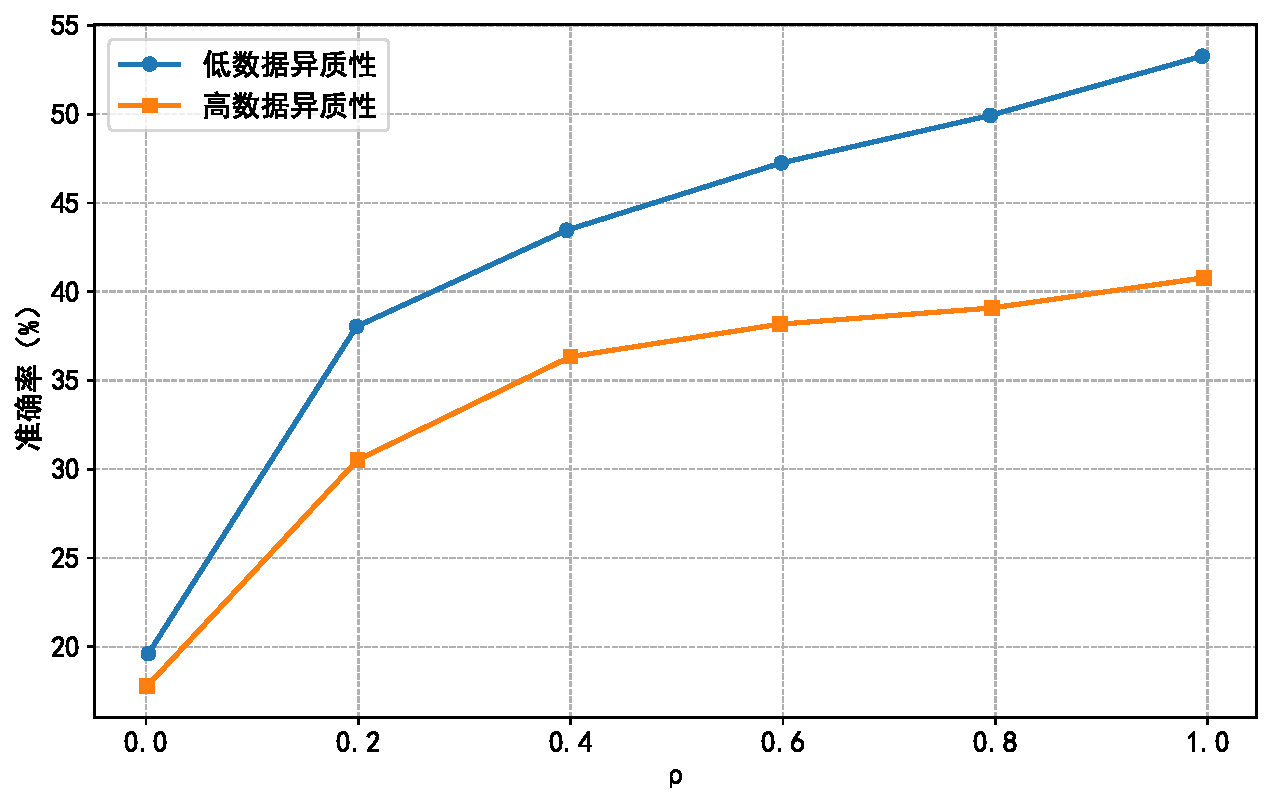
\includegraphics[width=0.9\linewidth]{chapter3/cifar10_rou.pdf}
    \caption{\label{fig:3-4-cifar-rou}CIFAR10上$\rho$对准确率影响曲线图}
\end{figure}
%ppppppppppppppppppppppppppppppppppppppp
表\ref{fig:3-4-cifar-rou}展示了在中等数据集CIFAR10上,分别在高低数据异质性下
$\rho$对模型准确率的影响。
在中等数据集CIFAR10上随着参数的增加,
模型的准确率随之增加。
低数据异质性准确率远高于高数据异质性场景,
与EMNIST的基本情况相似。
但是与之不同的是,
随着参数的增加中等数据集的准确率是一直增长的,
没有EMNIST上$\rho=0.2$的瓶颈,
在$\rho > 0.2$之后,模型的准确率也是逐步上升的,
增大模型的参数准确率还有上升的趋势。
这说明在中等数据集上,
无论是高数据异质性还是低数据异质性场景
参数数量是影响模型准确率的瓶颈,
通过提高训练模型的参数量就可以提高模型的准确率。
总结来说,
图\ref{fig:3-4-emnist-rou}和图\ref{fig:3-4-cifar-rou}
证明了在资源受限联邦学习的训练中特别是在任务比较复杂情况下,
训练的参数不够是影响模型准确率的重要因素,
可以增加训练模型的训练参数来提升模型能力。

\subsection{统计异质性的影响}
在上述实验中,我们定义了高低数据异质性。
也就是通过设定每位客户本地数据集中包含的训练数据的种类数
来确定数据的异质程度,
也就是客户端数据分布的均匀程度,
种类数越少意味着数据分布单一,均匀程度较差,训练难度大;
相反种类数量越大意味这数据分布均匀,模型泛化性好。
例如在EMNIST中高数据异质性的种类数是二,
低数据异质性的种类数是四,
如表\ref{tab:classinfo}所示。
本小节我们讨论客户端的数据异质性程度对于模型训练最终准确率的影响。
我们采用EMNIST数据集在简单的卷积神经网络上进行实验,
设定客户端的包含种类数分别为
$\{2, 4, 6, 8, 10 \}$。
%ppppppppppppppppppppppppppppppppppppppp
\begin{figure}[thbp]
    \centering
    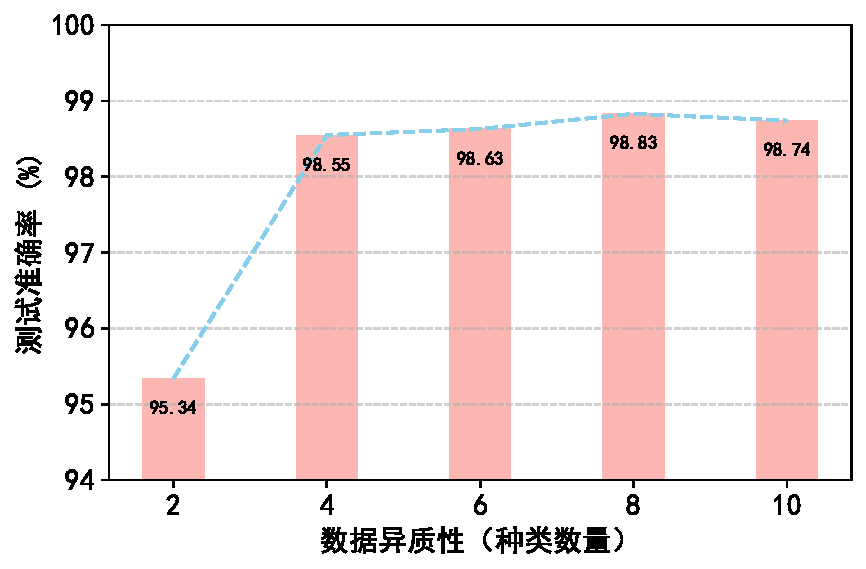
\includegraphics[width=0.9\linewidth]{chapter3/dataclass.pdf}
    \caption{\label{fig:3-4-dataclass}数据异质性对准确率的影响}
\end{figure}
%ppppppppppppppppppppppppppppppppppppppp

与参数多少对模型最终准确率的影响类似,
在简单数据集EMNIST上模型准确率对于数据分布均匀程度也存在一定的
阈值。
如图\ref{fig:3-4-dataclass}中所示,
在种类数为$2$的时候,训练的模型的准确率为$95.34\%$,
当种类数增加到$4$的时候,模型的准确率提升到$98.55\%$,
提升了$3.21\%$,
而当种类继续提高的时候,也就是数据更加均匀时,
模型的准确率依然在种类为4的结果附近徘徊,
没有得到大的提升。
这说明在简单任务上当数据均匀性增加到一定程度的时候,
模型的准确率增长会出现瓶颈。
在大多数实际情况中,
十分类问题中客户用到的也仅仅是四类,
这也符合实际情况,
也就是说我们的方法可以在实际中得到很好的应用。

\subsection{客户挑选比例对准确率的影响}
为了观察每轮中中心服务器挑选参与训练客户端比例对模型准确率的影响,
%ppppppppppppppppppppppppppppppppppppppp
\begin{figure}[thbp]
    \centering
    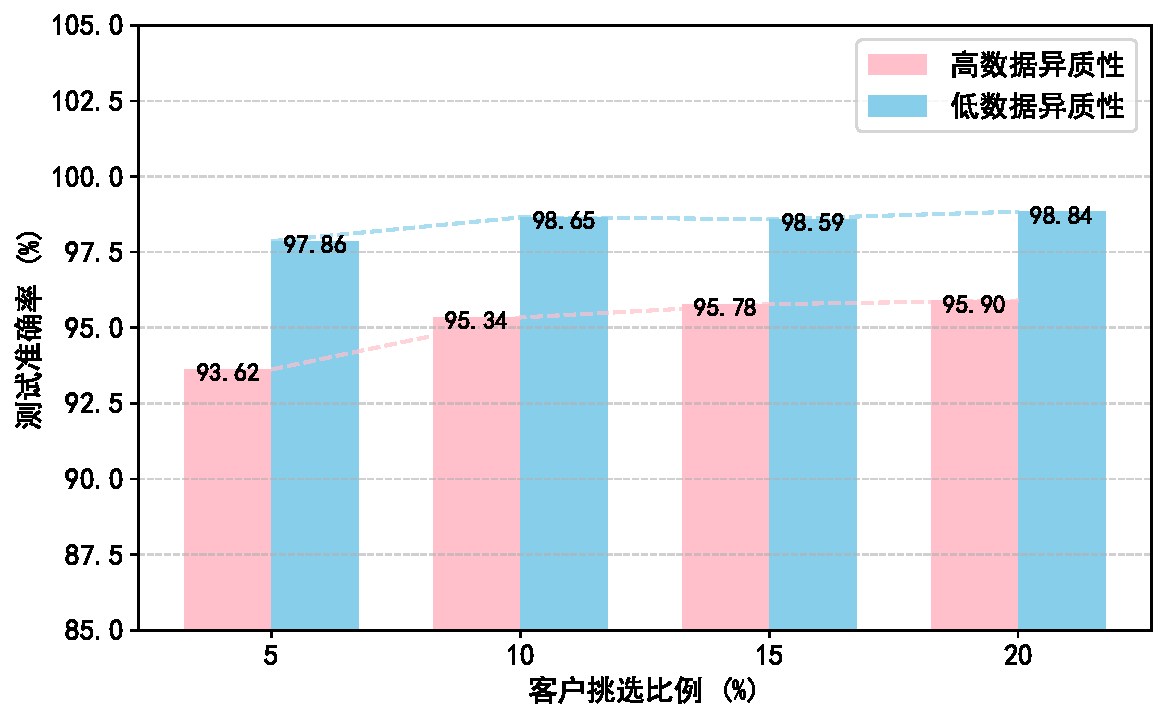
\includegraphics[width=0.9\linewidth]{chapter3/clientpor.pdf}
    \caption{\label{fig:3-4-clientpor}数据异质性对准确率的影响}
\end{figure}
%ppppppppppppppppppppppppppppppppppppppp
我们在简答数据集EMNIST上将挑选比例frc设定为
$\{5, 10, 15, 20 \}(\%)$,
分别在高数据异质和低数据异质情况下比较frc对模型准确率的影响。

如图\ref{fig:3-4-clientpor}所示高数据异质性情况下
当减小frc到$5\%$的时准确率仅有$93.62\%$,
而将frc提高到$10\%$时准确率提高到$95.34\%$,
此后增加每个轮次训练的客户的数量对模型准确率的增长效果不佳,
也就是说参加训练的客户端的数量也有一个阈值,
达到之后边际效应收紧。
同理这样的情况出现在低数据异质情况下,
由于低数据异质且是在简单数据集上进行实验,
frc的增加对模型准确率的影响没有在高数据异质情况下明显。
也就是说在$\text{frc}=5\%$的时候已经达到了低数据异质情况下的阈值。
通过上述分析我们观察到可以选择一个合适的frc的数值
使得既不增加模型训练的资源消耗,又能训练出与更多客户参与训练模型一样的效果。

\subsection{用于推理数据数量对准确率的影响}
在FedDSE中我们在抽取子模型过程中,首先要对全局模型进行推理,
然后再推理中通过激活值来选取每层抽取的神经元,
用来推理数据的大小对模型准确率也有很大的影响,
如算法\ref{alg:GetMaskFedDSE}中第二行中用来获取
$\mathbf{h}$中$\{x, y \}$的数量。
我们设定推理数量按照
$\{64, 128, 256, \text{all} \}$,
其中all表示整个完整本地数据集的数量。
同样在EMNIST数据集上,在高低数据异质性环境下进行实验。
%ppppppppppppppppppppppppppppppppppppppp
\begin{figure}[thbp]
    \centering
    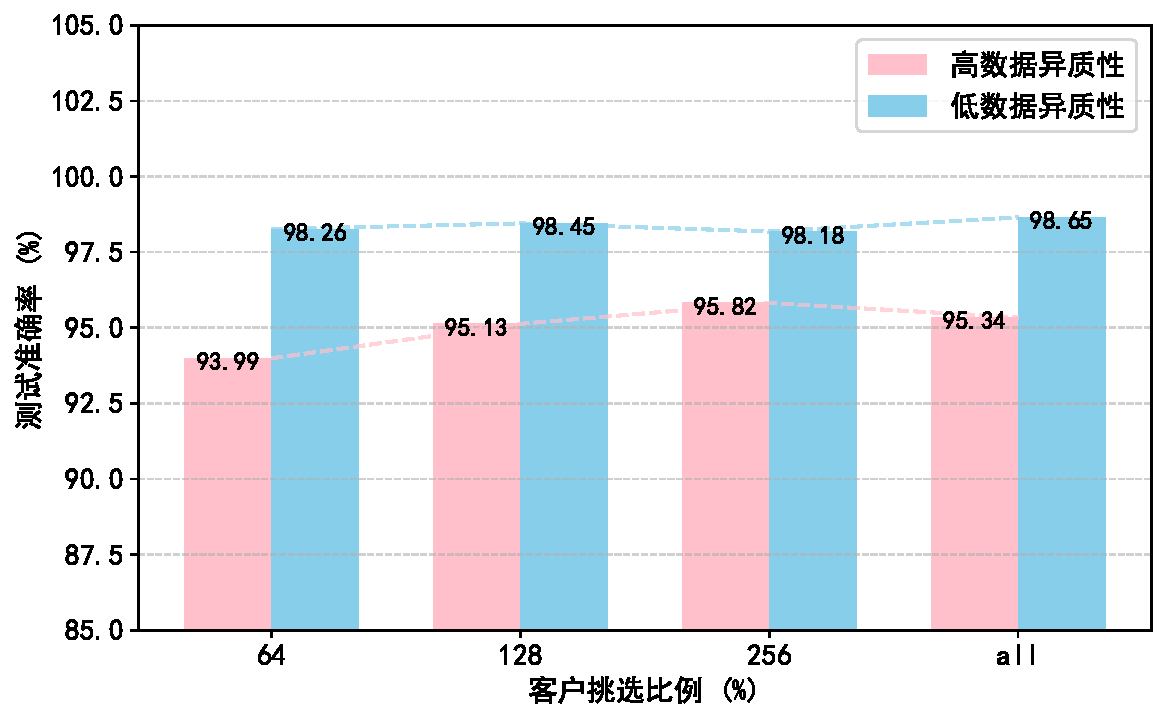
\includegraphics[width=0.9\linewidth]{chapter3/extract_size.pdf}
    \caption{\label{fig:3-4-extract_size}用于推理数据数量对准确率的影响}
\end{figure}
%ppppppppppppppppppppppppppppppppppppppp

具体结果如图\ref{fig:3-4-extract_size}所示,
在高数据集异质的情况下,
当推理数据的数量减少到$64$的时候,
模型的准确率下降到了$93.99\%$,
而当推理数据数量上升到$128$的时候,
模型的准确率上升到了$95.13\%$。
此后继续增加推理数量对模型的准确率影响较为不显著,
也就意味着使用128条数据对模型进行神经元抽取已经可以很好的
选择出活跃的神经元,
与增加推理数据情况下选择的神经元没有较大的差别。
然而这个现象在低数据异质性情况下不明显,
说明低数据异质情况下,
使用$64$条数据已经满足挑选活跃神经元需求,
所以模型的准确率没有发生大幅提升与下降。

\subsection{温度对模型准确率的影响}
在实际应用中,我们也可以自适应地选择温度,
以同时实现基于激活的选择和均衡训练选择的双重优势。
为验证这一点,我们还进行了实验,
将FedDSE与硬TopK和软TopK进行对比,
实验结果如表\ref{tab:effect_T}所示(基于 EMNIST 数据集)。
其中,
同构 (1/4)表示所有客户端都是同质的,
且只能训练完整模型的 $1/4$;
而异构能力(Heterogeneous capability)设置与表\ref{tab:total_high_res}
相同。
而数据异质性中的同分布是指数据遵循独立同分布,
也就是所有的客户端的数据分布相同。
\begin{table}[thbp]
    \caption{\label{tab:effect_T}温度对模型准确率的影响}
    \begin{tabularx}{\linewidth}{l l X<{\centering} X<{\centering} X<{\centering} }
        \toprule
        \multirow{2}{*}{模型计算能力} & \multirow{2}{*}{方法} & & 数据异质性 & \\
        \cline{3-5}
        & & 高 & 低 & 同分布 \\
        \midrule
        \multirow{3}{*}{同构 (1/4)} 
        & FedRolex & 93.35 & 97.29 & 97.04 \\
        & FedDSE (T=0) & 81.25 & 89.74 & 88.05\\
        & FedDSE (T=1) & \textbf{96.59} & \textbf{98.21} & \textbf{97.83} \\
        \midrule
        \multirow{3}{*}{同构 (1/2)}
        & FedRolex & 97.76 & 98.52 & 98.74 \\
        & FedDSE (T=0) & 91.51 & 96.53 & 95.24\\
        & FedDSE (T=1) & \textbf{98.45} & \textbf{99.16} & \textbf{99.09} \\
        \midrule
        \multirow{3}{*}{异构}
        &FedRolex & 91.41 & 98.61 & 98.67 \\
        &FedDSE (T=0) & \textbf{95.34} & \textbf{98.65} & \textbf{98.69}\\
        &FedDSE (T=1) & 94.60 & 97.86 & 98.15 \\
        \bottomrule
    \end{tabularx}
\end{table}

从表中可以观察到,$T=0$ 和 $T=1$ 在不同场景下分别表现更优。
通常情况下,较高的温度更适用于客户端能力均匀的场景,
例如在同构能力都为$1/4$的情况中,
温度$T=1$模型准确率的结果要远远好于当温度为$T=0$的时候,
特别是在高数据异质性的情况下,
提高了接近十五个百分点;
同样的情况还出现在同构模型能力为$1/2$情况下,
也是在高异质情况下提高了接近七个百分点。
而较低的温度则更适用于客户端能力不均的情况,
例如在我们异构情况下,也就是客户端均匀分布
$\mathbf{r} = \{ 0.99, 0.5, 0.25, 0.125, 0.0625 \}$
情况下,
$T=0$要比$T=1$效果更好。
此外,值得注意的是,我们的方法始终优于当前最先进的基线方法,即FedRolex。

\section{本章小结}
本文聚焦于联邦学习(Federated Learning, FL)中的子模型提取问题。
我们观察到,由于统计异质性,客户端倾向于激活模型的不同神经元。
这可能导致在不适当的子模型提取方式下,神经元之间出现竞争问题。
为了解决这一挑战,我们提出了一种新的联邦学习子模型提取方法,
该方法利用神经网络和边缘设备的激活分布特性,
通过选择激活值最大的神经元,自适应地将其分配给不同的客户端。
我们通过实验结果验证了其有效性,表现优于其他方法。
